\documentclass[12pt]{report}
\usepackage[thinc]{esdiff} % for typesettign derivatives
\usepackage{amsthm} % provides an enhanced version of LaTex's \newtheorem command
\usepackage{mdframed} % framed environments that can split at page boundaries
\usepackage{enumitem} % bulletin points or other means of listing things
\usepackage{amssymb} % for AMS symbols
\usepackage{amsmath} % so as to use align
\usepackage{latexsym} % so as to use symbols like \leadsto
\usepackage{mathrsfs} % for using mathscr for char like operators
\usepackage{commath} % for using norm symbol
\usepackage{mathtools} % for using environments like dcases
\usepackage{authblk} % for writing affiliations
\usepackage{graphicx} % for importing images
\graphicspath{{./images/}} % for the path to images, also always put label behind captions
\usepackage{textcomp} % for using degree symbol
\usepackage{hyperref} % for clickable link in the pdf & customizable reference text
\usepackage[all]{hypcap} % for clickable link to images instead of caption
\usepackage[margin=1in]{geometry} % default is 1.5in
% \usepackage[left=0.4in, right=0.4in, top=0.8in, bottom=0.8in]{geometry}
\usepackage[title]{appendix} % for attaching appendix
\allowdisplaybreaks % allow page breaking in display maths, like align
% allow for more advanced table layout
\usepackage{booktabs}
\usepackage{multirow}
\usepackage{siunitx}
% for adjusting caption settings
\usepackage{caption}
\captionsetup[table]{skip=10pt}

\theoremstyle{definition}
\mdfdefinestyle{defEnv}{%
  hidealllines=false,
  nobreak=true,
  innertopmargin=-1ex,
}

% The following is for writing block of code
\usepackage{listings}
\usepackage{color}

\definecolor{dkgreen}{rgb}{0,0.6,0}
\definecolor{gray}{rgb}{0.5,0.5,0.5}
\definecolor{mauve}{rgb}{0.58,0,0.82}

\setlength{\parindent}{0pt}
\setlength{\fboxrule}{2pt}

% Use the following to change code language and related settings
\lstset{frame=tb,
  language=Python,
  aboveskip=3mm,
  belowskip=3mm,
  showstringspaces=false,
  columns=flexible,
  basicstyle={\small\ttfamily},
  numbers=none,
  numberstyle=\tiny\color{gray},
  keywordstyle=\color{blue},
  commentstyle=\color{dkgreen},
  stringstyle=\color{mauve},
  breaklines=true,
  breakatwhitespace=true,
  tabsize=3
}

\pagestyle{headings}
\author{Lectured by Alex Geringer-Sameth}
\title{Probability and Statistics for JMC}
\affil{Typed by Aris Zhu Yi Qing}
\begin{document}
\maketitle
\tableofcontents

\chapter{Review of Elementary Set Theory}

\noindent\fbox{%
    \parbox{\textwidth}{%
        \begin{align*}
            \Omega & \qquad\text{universal set} \\
            \medskip
            \emptyset & \qquad\text{empty set} \\
            \medskip
            A\subseteq\Omega & \qquad\text{subset of $\Omega$} \\
            \medskip
            \overline{A} & \qquad\text{Complement of $A$} \\
            \medskip
            |A| & \qquad\text{cardinality of $A$} \\
            \medskip
            A\cup B & \qquad\text{union ($A$ or $B$)} \\
            \medskip
            A\cap B & \qquad\text{intersection($A$ and $B$)} \\
            \medskip
            A=B & \qquad\text{both sets have exactly the same elements} \\
            \medskip
            A\backslash B & \qquad\text{set difference (elements in $A$ that are
            not in $B$)} \\
            \medskip
            \left\{\omega\right\} & \qquad\text{a singleton with only the
            element $\omega$ in the set} \\
            \medskip
            A\times B & \qquad\left\{(a,b)|a\in A, b\in B\right\}
        \end{align*}  
    }%
}

\chapter{Visual and Numerical Summaries}

\section{Visualization}

\begin{figure}
  	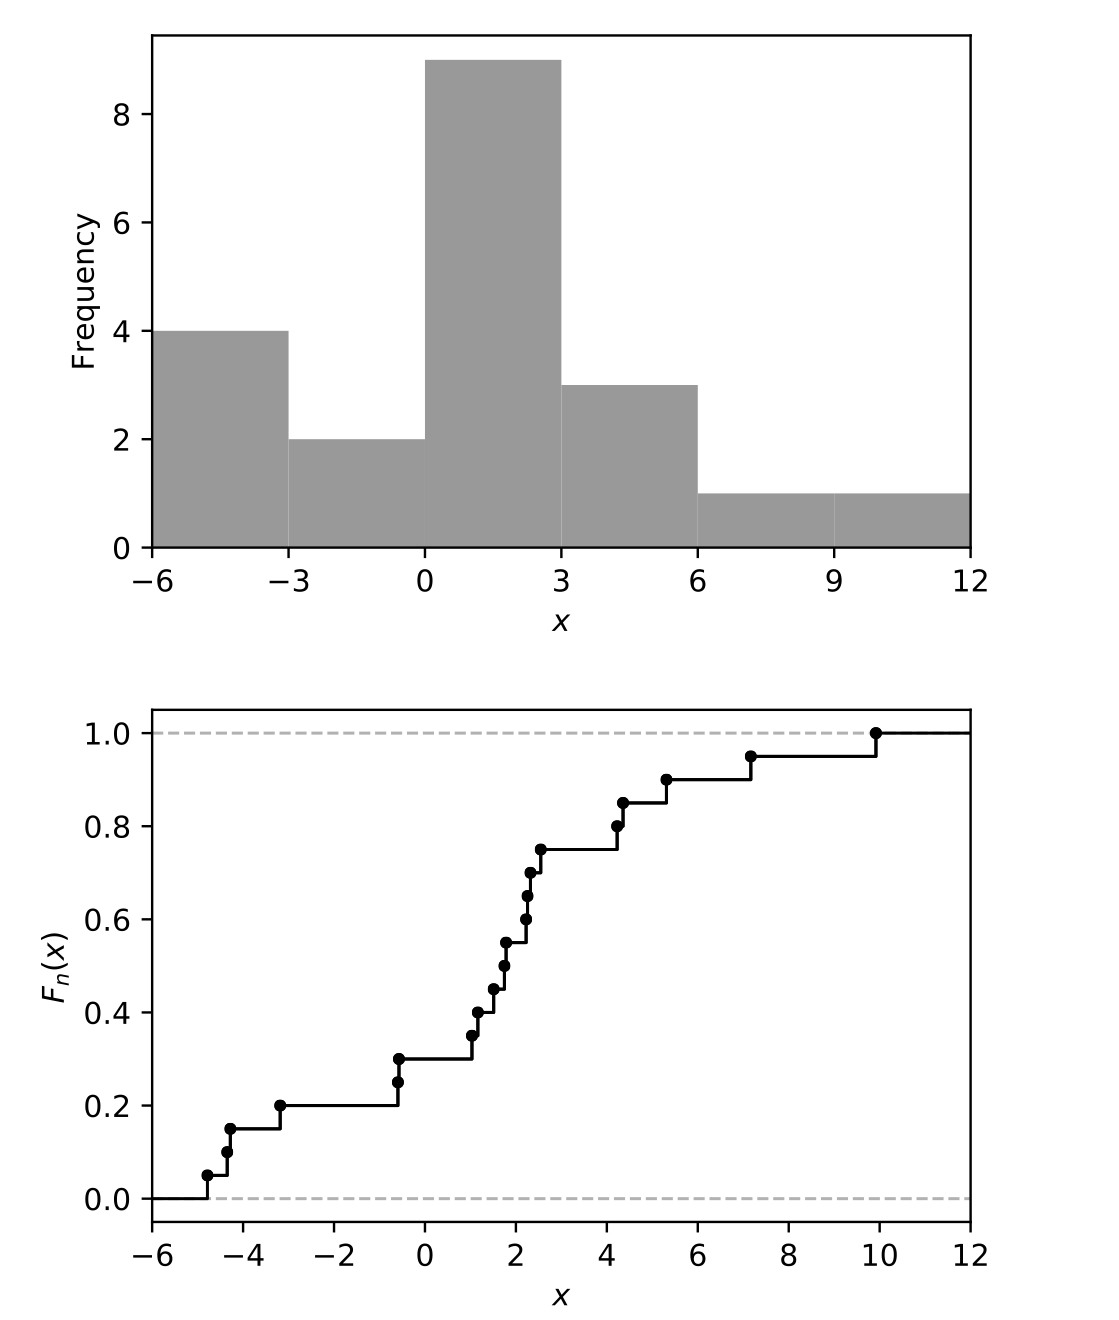
\includegraphics[scale=0.4]{./images/histogram_empirical_CDF.jpeg}
  	\centering
    \caption{The first diagram is the histogram, and the second diagram is the
    empirical cdf with the same set of data}\label{hist_cdf}
\end{figure}


\newmdtheoremenv[style=defEnv]{theorem}{Definition}
\begin{theorem}
The \textbf{\emph{histogram}} allows us to visualize how a sample of data
is distributed, say the observed values are $\left\{x_1,\ldots,x_2\right\}$.
The first step is deciding on a set of \textbf{\emph{bins}} that divide the
range of $x$ into a series of intervals.
A histogram then shows the \textbf{\emph{frequency}} for each bin.
\end{theorem}
\paragraph{\underline{Comments}}
Often the histogram's $y$-axis is normalized in some way.
\begin{itemize}
    \item 
        Instead of showing frequency, the height of the histogram can show
        \textbf{\emph{relative frequency}}, the fraction of the data set contained within the
        bin. 
        In this case, $1=\sum_{\text{bins }i} y_i$, where $y_i$ is the relative
        frequency at bin $i$.
    \item 
        The histogram could also show the \textbf{\emph{density}}, the relative
        frequency divided by the bin width.
        In this case, $1=\sum_{\text{bins }i} \rho_i\Delta x_i$, where $\rho_i$
        is the density for bin $i$ and $\Delta x_i$ is the width of bin $i$.
\end{itemize} 

\newmdtheoremenv[style=defEnv]{empirical CDF}[theorem]{Definition}
\begin{empirical CDF}
    The \textbf{\emph{empirical cumulative distribution function}} of a sample of
    real values $\left\{x_1,\ldots,x_n\right\}$ is
    \[
        F_n(x)=\frac{1}{n}\sum_{i=1}^{n} I(x_i\le x),
    \]
    where $I(x_i\le x)$ is an \textbf{\emph{indicator function}}, i.e.\ the
    value is 1 when $x_i\le x$ and 0 when $x_i>x$.
\end{empirical CDF}

\section{Summary Statistics}

\subsection{Measures of Location}

\noindent\fbox{%
    \parbox{\textwidth}{%
        \begin{align*}
            \text{arithmetic mean} & \qquad \overline{x}=\frac{1}{n}\sum_{i=1}^{n} x_i \\
            \text{geometric mean} & \qquad x_G={\left(\prod_{i=1}^{n}
            x_i\right)}^{\frac{1}{n}} \\
            \text{harmonic mean} &  \qquad\frac{1}{x_H}=\frac{1}{n}\sum_{i=1}^{n}
            \frac{1}{x_i} \\
            \text{$i^{\text{th}}$ order statistic} & \qquad x_{(i)}= \text{the
            $i^{\text{th}}$ smallest value of the sample} \\
            \text{median} &\qquad x_{\left(\frac{n+1}{2}\right)} \\
            \text{mode} & \qquad \text{$x_i$ which occurs most
            frequently in the sample}
        \end{align*} 
    }%
}
\paragraph{\underline{Comments}}
\begin{itemize}
        \item For positive data $\left\{x_1,\ldots,x_n\right\}$,
            \[
                \text{arithmetic mean}\ge\text{geometric mean}\ge\text{harmonic
                mean}.
            \]
        \item Arithmetic mean and geometric mean are related in the following
            way:
            \[
                \overline{x} = \frac{1}{n}\sum_{i=1}^{n} x_i =
                \frac{1}{n}\sum_{i=1}^{n} \ln{y_i} =
                \frac{1}{n}\ln{\prod_{i=1}^{n} y_i} =
                \ln{{\left(\prod_{i=1}^{n} y_i\right)}^{\frac{1}{n}}} =
                \ln{x_G},
            \]
            where $x_i = \ln{y_i}$.
        \item
            For $x_{(i)}$, when $i$ is not an integer, we define
            $\alpha\in(0,1)$ s.t. $\alpha=i-\lfloor i\rfloor $, and
            \[
                x_{(i)}=(1-\alpha)x_{(\lfloor i\rfloor)} 
                + \alpha x_{(\lceil i\rceil )}.
            \]
\end{itemize} 

\subsection{Measures of Dispersion}

\noindent\fbox{%
    \parbox{\textwidth}{%
        \begin{align*}
            \text{mean square/sample variance} & \qquad
            s^{2}=\frac{1}{n}\sum_{i=1}^{n} {(x_i-\overline{x})}^{2} \\
            \text{root mean square/sample standard deviation} & \qquad
            s = \sqrt{s^{2}} \\
            \text{range} & \qquad x_{(n)}-x_{(1)} \\
            \text{first quartile} & \qquad x_{\left(\frac{1}{4}(n+1)\right)} \\
            \text{third quartile} & \qquad x_{\left(\frac{3}{4}(n+1)\right)} \\
            \text{interquartile range} & \qquad 
            x_{\left(\frac{1}{4}(n+1)\right)} - x_{\left(\frac{3}{4}(n+1)\right)}
        \end{align*} 
    }%
}
\paragraph{Comments}
\begin{itemize}
        \item sample variance's different expression:
            \[
                s^{2} = \frac{1}{n}\sum_{i=1}^{n} {(x_i-\overline{x})}^{2}
                = \left(\frac{1}{n}\sum_{i=1}^{n} x_i^2\right)
                - {\left(\frac{1}{n}\sum_{i=1}^{n} x_i\right)}^{2}
                = \overline{x^{2}}-\overline{x}^{2}.
            \]
        \item Robustness, shown in table~\ref{robustness}
            \begin{table}[h]
                \centering
                \caption{Robustness of different location and dispersion statistic}
                \label{robustness}
                \begin{tabular}{l||c|c|c}
                    & Least Robust & More Robust & Most Robust \\
                    \hline\hline
                    Location & $\frac{x_{(1)}+x_{(n)}}{2}$ & $\overline{x}$ &
                    $x_{\left(\frac{n+1}{2}\right)}$ \\
                    \hline
                    Dispersion & $x_{(n)}-x_{(1)}$ & $s$ &
                    $x_{\left(\frac{3}{4}(n+1)\right)}-x_{\left(\frac{1}{4}(n+1)\right)}$
                \end{tabular} 
            \end{table} 
\end{itemize} 

\subsection{Covariance, Correlation, and Skewness}

\noindent\fbox{%
    \parbox{\textwidth}{%
        \begin{align*}
            \text{covariance} & \qquad s_{xy}=\frac{1}{n}\sum_{i=1}^{n}
            (x_i-\overline{x})(y_i-\overline{y}) \\
            \text{correlation} & \qquad r_{xy}=\frac{s_{xy}}{s_xs_y} \\
            \text{skewness} & \qquad \frac{1}{n}\sum_{i=1}^{n} 
            {\left(\frac{x_i-\overline{x}}{s}\right)}^{3}
        \end{align*} 
    }%
}
\paragraph{Comments}
\begin{itemize}
        \item covariance's different expression:
            \[
                s_{xy}=\frac{1}{n}\sum_{i=1}^{n}
                (x_i-\overline{x})(y_i-\overline{y})
                = \frac{1}{n}\sum_{i=1}^{n} x_iy_i+
                \frac{1}{n}\sum_{i=1}^{n} -x_i \overline{y}
                -\overline{x}y_i+\overline{x}\overline{y}
                = \frac{\sum_{i=1}^{n} x_iy_i}{n}
                -\overline{x}\,\overline{y}.
            \]
            In the random variable's context, it is
            \[
                \text{Cov}(X,Y)=E(XY)-E(X)E(Y).
            \]
        \item Correlation gives a \textbf{scale-invariant}
            measurement of relatedness between $x$ and $y$, since
            \[
                |r_{xy}|\le 1.
            \]
        \item A sample is \textbf{positively (negatively)} or
            \textbf{right (left) skewed} if the upper tail of the histogram of
            the sample is longer (shorter) than the lower tail.
\end{itemize} 

\subsection{Box-and-whisker plot}

The diagram is based on the five-point summary (use Figure~\ref{box-plot} as
reference):
\begin{itemize}
    \item Median -- middle line in the box.
    \item 3\textsuperscript{rd} and 1\textsuperscript{st} Quartiles -- top and
        bottom of the box.
    \item ``Whiskers'' -- extend out as dashed lines from the box to max/min
        values, which are the two short horizontal lines.
    \item Any outliers, i.e.\ extreme points beyond the whiskers, are plotted
        individually as dots.
\end{itemize} 
\begin{figure}[h]
  	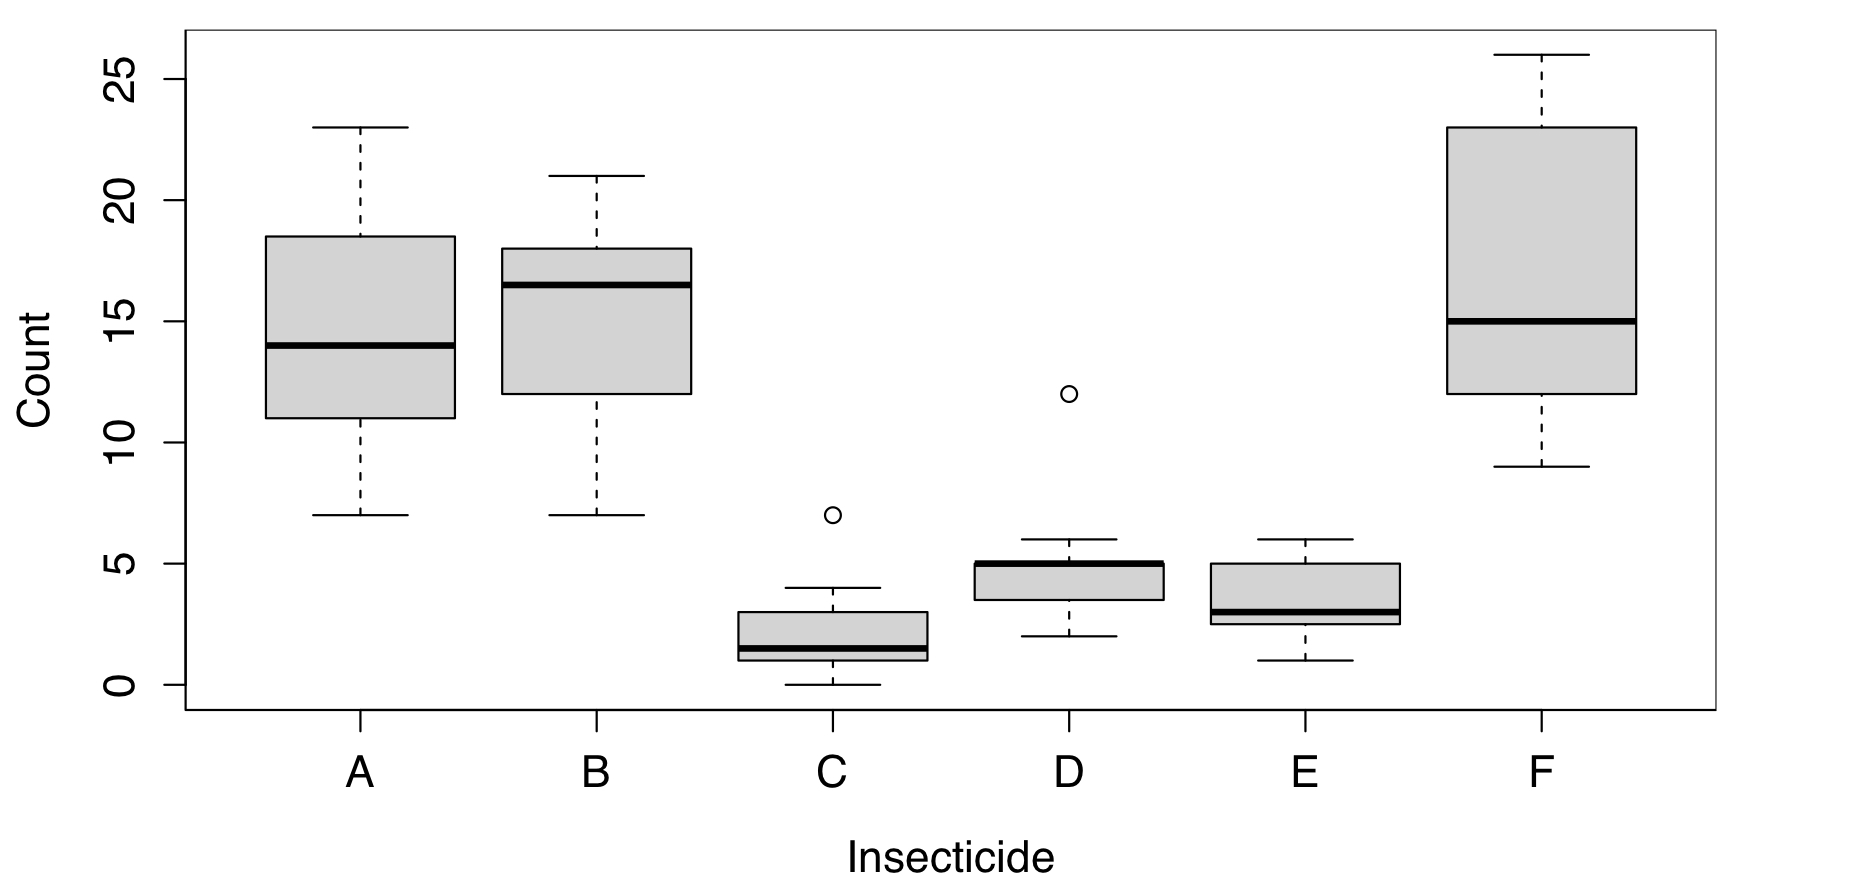
\includegraphics[scale=0.18]{./images/box-and-whisker.jpeg}
  	\centering
  	\caption{the counts of insects found in agricultural experimental units
    treated with six different insecticides A-F}\label{box-plot}
\end{figure}

\chapter{Probability}

\section{Formal Definition of Probability}

\subsection{$\sigma$-algebra}

\newmdtheoremenv[style=defEnv]{sigma algebra}[theorem]{Definition}
\begin{sigma algebra}\label{sigma-algebra}
    $\mathcal{F}$, a collection of subsets of a set $S$,
    is called a \textbf{\emph{$\sigma$-algebra}} associated with
    $S$ if:
    \begin{enumerate}[label = (\alph*)]
        \item $S\in\mathcal{F}$,
        \item $\mathcal{F}$ is closed under complements w.r.t. $S$:
            \[
                E\in\mathcal{F} \Longrightarrow \overline{E}\in\mathcal{F},
            \]
        \item $\mathcal{F}$ is closed under countable unions:
            \[
                E_1,E_2,\ldots\in\mathcal{F}\Longrightarrow
                \bigcup_{i=1}^{\infty}E_i\in\mathcal{F}.
            \]
    \end{enumerate} 
\end{sigma algebra}

\paragraph{Comments}
Definition~\ref{sigma-algebra} implies two facts.
\begin{enumerate}
    \item $\mathcal{F}$ must contain the empty set $\emptyset$.
        \begin{proof}
            Since $S\in\mathcal{F}$, we have
            $\overline{S}=\emptyset\in\mathcal{F}$.
        \end{proof} 
    \item $\mathcal{F}$ must be closed under countable intersections.
        \begin{proof}
            Let $E_1,E_2,\ldots\in\mathcal{F}$. We can then imply the following:
            \[
                \overline{E_1},\overline{E_2},\ldots\in\mathcal{F}
                \Rightarrow \bigcup_i \overline{E_i}\in\mathcal{F}
                \Rightarrow \overline{\bigcup_i \overline{E_i}}\in\mathcal{F}
                \xrightarrow{\text{De Morgan's Law}}\bigcap_iE_i\in\mathcal{F}.
            \]
        \end{proof} 
\end{enumerate} 
In short, we can take unions, intersections, and complements of members of
$\mathcal{F}$ in any combination and the result will always be a member of
$\mathcal{F}$.

\subsection{Probability Measure}

\newmdtheoremenv[style=defEnv]{probability measure and space}[theorem]
{(Kolmogorov's axioms of probability) Definition}
\begin{probability measure and space}
    A \textbf{\emph{probability measure}} $P$ is a function
    $P:\mathcal{F}\mapsto\mathbb{R}$ satisfying
    \begin{enumerate}[label = (\alph*)]
        \item $P(E)\ge 0 \;\forall E\in\mathcal{F}$,
        \item $P(S)=1$,
        \item If $E_1,E_2,\ldots\in\mathcal{F}$ are disjoint (i.e.\ $E_i\cap
            E_j=\emptyset \;\forall i\neq j$) then
            \[
                P\left(\bigcup_{i=1}^{\infty}E_i\right)=
                \sum_{i=1}^{\infty} P(E_i).
            \]
    \end{enumerate} 
    The triplet $(S,\mathcal{F},P)$, consisting of a set $S$, a $\sigma$-algebra
    $\mathcal{F}$ of subsets of $S$, and a probability measure $P$, is called a
    \textbf{\emph{probability space}}.
\end{probability measure and space}

\paragraph{Comments}
\begin{itemize}
    \item The \textbf{\emph{sample space}} $(S)$ is the set of all possible
        outcomes of an experiment.
    \item The \textbf{\emph{event space}} $(\mathcal{F})$ is the set of possible
        events, where an \textbf{\emph{event}} $E$ is a subset of the sample
        space, $E\subseteq S$. An \textbf{\emph{elementary event}} is one that
        consist of a single element of $S$, i.e.\ a singleton.
    \item The probability measure $(P)$ has three important interpretations:
        \begin{enumerate}
            \item \textbf{classical}:
                Different outcomes in the sample space $S$ 
                are ``equally likely'',
            \item \textbf{frequentist}:
                the relative frequency of an event over many trials,
            \item \textbf{subjective}:
                a numerical measure of the degree of belief held by an individual.
        \end{enumerate} 
        \newtheorem{probability-interpretations}[theorem]{Example}
        \begin{probability-interpretations}
            ``A sensor can detect items within 10 cm of the sensor.
            The sensor is placed in a room together with an object, and
            the probability that the sensor makes a detection is 0.0001.''
            \begin{enumerate}
                \item \textbf{classical}:
                    The volume within 10 cm of the sensor divided by the volume
                    of the room is 0.0001.
                \item \textbf{frequentist}:
                    If we repeat the experiment a lot of times, then the
                    fraction of the experiments in which the sensor makes a
                    detection is 0.0001.
                \item \textbf{subjective}:
                    Someone's subjective degree of belief, measured on a
                    numerical scale from 0 to 1, that the sensor will detect is
                    0.0001.
            \end{enumerate} 
        \end{probability-interpretations}
    \item several results that can be derived from the probability measure
        axioms:
        \begin{itemize}
            \item $P(\emptyset)=0$.
            \item $P(E)\le 1$.
            \item $P(\overline{E})=1-P(E)$.
            \item $P(E\cup F)=P(E)+P(F)-P(E\cap F)$..
            \item $P(E\cap \overline{F})=P(E)-P(E\cap F)$.
            \item If $E\subset F$ then $P(E)\le P(F)$.
        \end{itemize} 
\end{itemize} 

\section{Conditional Probability}

\newmdtheoremenv[style=defEnv]{conditional probability}[theorem]{Definition}
\begin{conditional probability}
    If $P(F)>0$ then the \textbf{\emph{conditional probability}} of $E$ given
    $F$ is
    \[
        P(E|F)=\frac{P(E\cap F)}{P(F)}.
    \]
\end{conditional probability}
\paragraph{Comments}
\begin{itemize}
    \item Difference among the following forms:
        \begin{itemize}
            \item $P(E|F)$ -- \textbf{\emph{conditional probabilities}},
            \item $P(E\cap F)$ -- \textbf{\emph{joint probabilities}},
            \item $P(E)$ -- \textbf{\emph{marginal probabilities}}.
        \end{itemize} 
    \item several results derived from the conditional probability definition:
        \begin{itemize}
            \item $P(E|F)\ge 0$ for any event $E$.
            \item $P(F|F)=1$.
            \item If the events $E_1,E_1,\ldots$ are pairwise disjoint, then
                $P\left(\left(\bigcup_i E_i\right)|F\right)=\sum_{i} P(E_i|F)$.
        \end{itemize} 
    \item \underline{Warning}: In general, $P(E|F)\neq P(F|E)$.
\end{itemize} 

\newtheorem{conditional probability eg}[theorem]{Example}
\begin{conditional probability eg}
    A medical test for a disease $D$ has outcomes $+$ and $-$.
    The probabilities are
    \begin{table}[h]
        \centering
        \begin{tabular}{l||c|c|c}
            & $D$ & $\overline{D}$ & \\
            \hline\hline
            $+$ & 0.009 & 0.099 & 0.108 \\
            \hline
            $-$ & 0.001 & 0.891 & 0.892 \\
            \hline
                & 0.01 & 0.99 &
        \end{tabular} 
    \end{table} 

    By the definition of conditional probability, we have
    \[
        P(+|D)=90\%,\quad P(-|\overline{D})=90\%, \quad
        P(D|+)=\frac{0.009}{0.108}\approx 0.083.
    \]
    The first two probabilities show that the test is fairly accurate. Sick
    people yield a positive 90\% of the time and healthy people yield a negative
    90\% of the time.
\end{conditional probability eg}


\section{Independence}

\newmdtheoremenv[style=defEnv]{independence}[theorem]{Definition}
\begin{independence}
    Two events $E$ and $F$ are \textbf{\emph{independent}} iff
    \[
        P(E\cap F)=P(E)P(F).
    \]
\end{independence}
\paragraph{Comments}
\begin{itemize}
    \item Extension: The events $E_1,\ldots,E_k$ are independent if, for every
        subset of events of size $l\le k$, say indexed by
        $\left\{i_1,\ldots,i_l\right\}$,
        \[
            P\left(\bigcap_{j=1}^l E_{i_j}\right)=\prod_{j=1}^{l} P(E_{i_j}).
        \]
    \item Independence could be either assumed or verified via the definition.
    \item Disjoint events with positive probability are not independent.
    \item From the definition of conditional probability, we can deduce that
        $E$ and $F$ are independent iff $P(E|F)=P(E)$.
\end{itemize} 

\newmdtheoremenv[style=defEnv]{conditional independence}[theorem]{Definition}
\begin{conditional independence}
    For three events $E_1, E_2, F$, the pair of events $E_1$ and $E_2$ are
    said to be \textbf{\emph{conditionally independent given $F$}} iff
    \[
        P(E_1\cap E_2|F) = P(E_1|F)P(E_2|F).
    \]
    which could also be written as $E_1\bot E_2|F$.
\end{conditional independence}

\section{Bayes' Theorem}

\newmdtheoremenv[style=defEnv]{law of total probability}[theorem]{(The Law of
Total Probability) Theorem}
\begin{law of total probability}
    Let $E_1,E_2,\ldots$ be a partition of $S$,
    i.e.\ $E_i\cap E_j=\emptyset$ for $i\neq j$ and $\bigcup_i E_i=S$.
    Then, for any event $F\subseteq
    S$, we have
    \[
        P(F)=\sum_{i}P(F|E_i)P(E_i).
    \] 
\end{law of total probability}
\begin{proof}
    $P(F)=P(\bigcup_i F\cap E_i)=\sum_{i} P(F\cap E_i)=\sum_{i}P(F|E_i)P(E_i)$.
\end{proof} 

\newmdtheoremenv[style=defEnv]{bayes' theorem}[theorem]{(Bayes' Theorem) Theorem}
\begin{bayes' theorem}
    If $P(F)>0$ and let $E_1,E_2,\ldots$ be a partition on $S$ s.t. $P(E_i)>0
    \,\forall i$, we have
    \[
        P(E_i|F)=\frac{P(F|E_i)P(E_i)}{P(F)}
        = \frac{P(F|E_i)P(E_i)}{\sum_{j}P(F|E_j)P(E_j)},
    \]
    where $P(E_i|F)$ is called the \textbf{\emph{posterior}},
    $P(F|E_i)$ is called the \textbf{\emph{likelihood}},
    $P(E_i)$ is called the \textbf{\emph{prior}},
    and $P(F)$ is called the \textbf{\emph{evidence}}.
\end{bayes' theorem}
\begin{proof}
    Exercise! haha
\end{proof} 

\newtheorem{bayes' theorem eg}[theorem]{Example}
\begin{bayes' theorem eg}
    A new covid-19 test is claimed to correctly identify 95\% of people who are
    really covid-positive and 98\% of people who are really covid-negative.
    If only 1 in a 1000 of the population are infected, what is the probability
    that a randomly selected person who tests positive actually has the disease?

    \medskip
    Let $I$ = ``has a covid infection'' and $T$ = ``test is positive''.
    We are given $P(T|I)=0.95,P(\overline{T}|\overline{I})=0.98,P(I)=0.001$.
    We can thus derive that
    \[
        P(I|T)=\frac{P(T|I)P(I)}{P(T)}
        =\frac{P(T|I)P(I)}{P(T|I)P(I)+P(T|\overline{I})P(\overline{I})}
        = \frac{0.95\times 0.001}{0.95\times 0.001 + 0.02\times 0.999}
        = 0.045.
    \]
\end{bayes' theorem eg}

\chapter{Discrete Random Variables}

\section{Random Variables}

\newmdtheoremenv[style=defEnv]{random variable}[theorem]{Definition}
\begin{random variable}
    A \textbf{\emph{random variable}} is a (measurable) mapping
    \[
        X:S\mapsto\mathbb{R}
    \]
    with the property that 
    $\left\{s\in S:X(s)\le x\right\}\in\mathcal{F}\;\forall x\in\mathbb{R}$.
    This ensures that any set $B\subseteq\mathbb{R}$ corresponds to an event in
    the event space $\mathcal{F}$.
\end{random variable}

\newmdtheoremenv[style=defEnv]{range of X}[theorem]{Definition}
\begin{range of X}
    The image of $S$ under $X$ is called the \textbf{\emph{range}} of the random
    variable
    \[
        \mathbb{X}\equiv X(S)=\left\{X(s)|s\in S\right\}
        =\left\{x\in\mathbb{R}\,|\,\exists s\in S\text{ s.t. }X(s)=x\right\}.
    \]
    So $S$ contains all the possible outcomes of the experiment, 
    $\mathbb{X}$ contains all the possible outcomes of the random variable $X$.
\end{range of X}

\newmdtheoremenv[style=defEnv]{probability distribution}[theorem]{Definition}
\begin{probability distribution}
    The \textbf{\emph{probability distribution}} of $X$ is defined as
    \[
        P_X = P_X(X\in B\subseteq\mathbb{R}) 
        = P(\left\{s\in S:X(s)\in B\right\})
    \]
    which enables us to transfer the probability measure $P$ defined on $\mathcal{F}$
    to the real numbers in a natural way, and vice versa. For instance,
    \begin{align*}
        P_X(X=7) & = P(\left\{s\in S|X(s) = 7\right\}), \\
        P_X(a<X\le b) & = P(\left\{s\in S|a<X(s)\le b\right\}).
    \end{align*} 
\end{probability distribution}

\newtheorem{probability distribution application eg}[theorem]{Example}
\begin{probability distribution application eg}
    Consider counting the number of heads in a sequence of 3 coin tosses. The
    underlying sample space is
    \[
        S = \left\{TTT,TTH,THT,HTT,THH,HTH,HHT,HHH\right\}.
    \]
    Since we are only interested in the number of heads in each sequence,
    we define the random variable $X$ by
    \[
        X(s)=
        \begin{cases}
            0, & s=TTT,\\
            1, & s\in\left\{TTH,THT,HTT\right\}, \\
            2, & s\in\left\{HHT,HTH,THH\right\}, \\
            3, & s=HHH.
        \end{cases} 
    \]
    Thus, the probability of the number of heads $X$ is less than 2 is
    \begin{align*}
        P_X(X<2)
        & =P(\left\{s\in S:X(s)<2\right\}) \\
        & =P(\left\{TTT,TTH,THT,HTT\right\}) \\
        & =\frac{\left|\left\{TTT,TTH,THT,HTT\right\}\right|}{|S|} \\
        & =\frac{4}{8}= \frac{1}{2}.
    \end{align*} 
    On a side note, the above process uses the classical interpretation on the
    probability measure.
\end{probability distribution application eg}

\newmdtheoremenv[style=defEnv]{cdf}[theorem]{Definition}
\begin{cdf}
    The \textbf{\emph{Cumulative Distribution Function (CDF)}} of a random
    variable $X$ is the function $F_X:\mathbb{R}\mapsto[0,1]$, defined by
    \[
        F_X(x)=P_X(X\le x)=P(\left\{s\in S:X(s)\le x\right\}).
    \]
\end{cdf}
\paragraph{Comments}
\begin{itemize}
    \item Given a right-continuous function $F_X(x)$, check the following to
        verify if it is a valid CDF:
        \begin{enumerate}[label = (\roman*)]
            \item $0\le F_X(x)\le 1\;\forall x\in\mathbb{R}$,
            \item Monotonicity (non-decreasing):
                $\forall x_1,x_2\in\mathbb{R}, x_1<x_2\Rightarrow F_X(x_1)\le
                F_X(x_2)$.
            \item $F_X(-\infty)=0, F_X(\infty)=1$.
        \end{enumerate} 
    \item For finite intervals $(a,b]\subseteq\mathbb{R}$, it is easy to check
        that 
        \[
            P_X(a<X\le B)=F_X(b)-F_X(a).
        \]
    \item Usually we suppress the subscript of $P_X(\cdot)$ and just write
        $P(\cdot)$ for the probability measure for the random variable, unless
        there is any ambiguity.
\end{itemize} 

\section{Discrete Random Variables}

\newmdtheoremenv[style=defEnv]{discrete RV}[theorem]{Definition}
\begin{discrete RV}
    A random variable $X$ is \textbf{\emph{discrete}} if the range of $X$,
    $\mathbb{X}$, is countable, that is
    \[
        \mathbb{X}=\left\{x_1,x_2,\ldots,x_n\right\}\text{ (finite)}
        \quad\text{or}\quad 
        \mathbb{X}=\left\{x_1,x_2,\ldots\right\}\text{ (infinite)}.
    \]
\end{discrete RV}

\newmdtheoremenv[style=defEnv]{pmf}[theorem]{Definition}
\begin{pmf}
    For a discrete random variable $X$, we define the \textbf{\emph{Probability
    Mass Function (PMF)}} as\[
        p_X(x)=P_X(X=x),\quad x\in\mathbb{X}.
    \]
    For completeness, we also define
    \[
        p_X(x) = 0, \quad x\notin\mathbb{X}.
    \]
    so that $p_x$ is defined for all $x\in\mathbb{R}$.
\end{pmf}

\newmdtheoremenv[style=defEnv]{support}[theorem]{Definition}
\begin{support}
    The \textbf{\emph{support}} of a random variable $X$ is defined as
    \[
        \left\{x\in\mathbb{R}: p_X(x)>0\right\},
    \]
    which is \underline{almost always} the same as the range $\mathbb{X}$.
\end{support}

\subsubsection{Properties of $p_X$ and $F_X$}
\begin{itemize}
    \item $p_X(x_i)\ge 0$.
    \item $\sum_{x\in\mathbb{X}} p_X(x)=1$.
    \item $F_X(x)=P(X\le x)$, $x\in\mathbb{R}$.
    \item Let $X$ be a discrete random variable with range
        $\mathbb{X}=\left\{x_1,x_2,\ldots\right\}$, where $x_1<x_2<\ldots$.
        Then for any $x\in\mathbb{R}$, if $x<x_1$, $F_X(x)=0$; otherwise
        \[
            F_X(x)=\sum_{x_i\le x} p_X(x_i) \iff p_X(x_i)=F_X(x_i)-F_X(x_{i-1}),
                \quad i=2,3,\ldots,
        \]
        with $p_X(x_1)=F_X(x_1)$.
    \item $\lim_{x\rightarrow-\infty}F_X(x)=0$,
        $\lim_{x\rightarrow\infty}F_X(x)=1$.
    \item $F_X$ is continuous from the right on $\mathbb{R}$, i.e.\ for
        $x\in\mathbb{R}$, $\lim_{h\rightarrow 0^{+}}F_X(x+h)=F_X(x)$.
    \item $F_X$ is non-decreasing, i.e.\
        $a<b \Longrightarrow F_X(a)\le F_X(b)$.
    \item For $a<b$, $P(a<X\le b)=F_X(b)-F_X(a)$.
\end{itemize} 

\section{Functions of a Discrete Random Variable}

\newmdtheoremenv[style=defEnv]{pmf of g(X)}[theorem]{Definition}
\begin{pmf of g(X)}
    The PMF of $Y=g(X)$ is found by grouping all the values in the range of $x$
    that correspond to the same value of $Y$, i.e.\
    \[
        p_{Y}(y)=\sum_{x\in\mathbb{X}:g(x)=y} p_X(x).
    \]
\end{pmf of g(X)}

\section{Mean and Variance}

\newmdtheoremenv[style=defEnv]{mean}[theorem]{Definition}
\begin{mean}
    The \textbf{\emph{expected value}}, or \textbf{\emph{mean}} of a discrete
    random variable $X$ is defined to be 
    \[
        E_X(X)=\sum_{x\in\mathbb{X}} xp_X(x),
    \]
    which is often written as $E(X)$, $E[X]$, or $\mu_X$.
\end{mean}

\newmdtheoremenv[style=defEnv]{E(g(X))}[theorem]{Theorem}
\begin{E(g(X))}
    \[
        E(g(X))=\sum_{x\in\mathbb{X}} g(x)p_X(x).
    \]
\end{E(g(X))}
\begin{proof}
    Let $Y=g(X)$, then
    \begin{align*}
        E(Y) & = \sum_{y\in \mathbb{Y}} yp_Y(y) \\
             & = \sum_{y\in \mathbb{Y}} y \sum_{x\in\mathbb{X}:g(x)=y} p_X(x) \\
             & = \sum_{y\in \mathbb{Y}} \sum_{x\in\mathbb{X}:g(x)=y} g(x)p_X(x) \\
             & = \sum_{x\in\mathbb{X}} g(x)p_X(x).
    \end{align*} 
\end{proof} 

\newmdtheoremenv[style=defEnv]{linearity of expectation}[theorem]{Theorem}
\begin{linearity of expectation}
    Let $X$ be a random variable with $p_X$. Let $g$ and $h$ be real-valued
    functions, $g,h:\mathbb{R}\mapsto\mathbb{R}$, and let $a$ and $b$ be
    constants. Then
    \[
        E(ag(X)+bh(X)) = aE(g(X))+bE(h(X)).
    \]
\end{linearity of expectation}
\begin{proof}
    Exercise!
\end{proof} 

\newmdtheoremenv[style=defEnv]{variance}[theorem]{Definition}
\begin{variance}
    Let $X$ be a random variable. The \textbf{\emph{variance}} of $X$, denoted
    by $\sigma^{2}$ or $\sigma_X^{2}$ or $\text{Var}_X(X)$,
    is defined by
    \[
        \text{Var}_X(X)=E_X\left[{(X-E_X(X))}^{2}\right].
    \]
\end{variance}

\newmdtheoremenv[style=defEnv]{variance alternate form}[theorem]{Proposition}
\begin{variance alternate form}
    \[
        \text{Var}(X)=E(X^{2})-E(X)^{2}.  
    \]
\end{variance alternate form}
\begin{proof}
    \begin{align*}
        \text{LHS} & = E\left[X^{2}-2E(X)X+E(X)^{2}\right] \\
                   & = E(X^{2})-2E(X)E(X)+E(X)^{2} \\
                   & = \text{RHS}.
    \end{align*} 
\end{proof} 

\newmdtheoremenv[style=defEnv]{variance of sum of two RV}[theorem]{Proposition}
\begin{variance of sum of two RV}
    \[
        \text{Var}(aX\pm bY) = a^{2}\text{Var}(X)
        + b^{2}\text{Var}(Y) \pm 2ab\text{Cov}(X,Y).
    \]
\end{variance of sum of two RV}
\begin{proof}
    Exercise!
\end{proof} 

\newmdtheoremenv[style=defEnv]{standard deviation}[theorem]{Definition}
\begin{standard deviation}
    The \textbf{\emph{standard deviation}} of a random variable $X$, written
    $\text{sd}_X(X)$ or $\sigma_X$, is the square root of the variance,
    \[
        \sigma_X = \sqrt{\text{Var}_X(X)}.
    \]
\end{standard deviation}

\newmdtheoremenv[style=defEnv]{skewness of discrete RV}[theorem]{Definition}
\begin{skewness of discrete RV}
    The \textbf{\emph{skewness}} ($\gamma_1$) of a discrete random variable $X$
    is given by
    \[
        \gamma_1=\frac{E_X\left[{\left\{X-E_X(X)\right\}}^{3}\right]}{\sigma_X^{3}}.
    \]
\end{skewness of discrete RV}

\subsubsection{Sums of Random Variables}

Let $X_1,X_2,\ldots,X_n$ be $n$ random variables, perhaps with different
distributions and not necessarily independent. Let $S_n=\sum_{i=1}^{n} X_i$ be
the sum of those variables, and $\frac{S_n}{n}$ be their sample average. Both
$S_n$ and $\overline{S}=\frac{S_n}{n}$ are random variables themselves.

\bigskip
The mean of $S_n$ and $\frac{S_n}{n}$ are given by
\[
    E(S_n)=\sum_{i=1}^{n} E(X_i),\quad 
    E\left(\overline{S}\right)=\frac{\sum_{i=1}^{n} E(X_i)}{n}=\mu_X.
\]

If $X_1,X_2,\ldots,X_n$ are \textbf{independent}, we can calculate the variance
of $S_n$ and $\overline{S}=\frac{S_n}{n}$ as well:
\[
    \text{Var}(S_n)=\sum_{i=1}^{n} \text{Var}(X_i),\quad
    \text{Var}(\overline{S})=\frac{\sum_{i=1}^{n}
    \text{Var}(X_i)}{n^{2}}=\frac{\sigma_X^{2}}{n}.
\]

\section{Some important Discrete Random Variables}

\newmdtheoremenv[style=defEnv]{bernoulli distribution}[theorem]{Definition}
\begin{bernoulli distribution}
    We say $X$ follows a \textbf{\emph{Bernoulli Distribution}} if $X\sim 
    \text{Bernoulli}(p)$, where $0\le p\le 1$, and the pmf is given by
    \[
        p_X(x)=
        \begin{cases}
            p & x=1 \\
            1-p & x=0 \\
            0 & \text{otherwise}
        \end{cases} 
        = p^{x}{(1-p)}^{1-x}, \quad x\in\mathbb{X}=\left\{0,1\right\}.
    \]
\end{bernoulli distribution}

\newmdtheoremenv[style=defEnv]{bionomial distribution}[theorem]{Definition}
\begin{bionomial distribution}
    We say $X$ follows a \textbf{\emph{Binomial Distribution}} if $X\sim
    \text{Binomial}(n, p)$, where $0\le p \le 1$ and $n\in\mathbb{Z}^+$, 
    and the pmf is given by
    \[
        p_{X}(x)=\begin{pmatrix}
                n \\
                x
            \end{pmatrix} p^{x}{(1-p)}^{n-x}, \quad
            x\in\mathbb{X}=\left\{0,1,2,\ldots,n\right\}.
    \]
\end{bionomial distribution}

\newmdtheoremenv[style=defEnv]{geometric distribution}[theorem]{Definition}
\begin{geometric distribution}
    We say $X$ follows a \textbf{\emph{Geometric Distribution}} if $X\sim
    \text{Geometric}(p)$, where $0\le p\le 1$, and the pmf is given by
    \[
        p_{X}(x)=p{(1-p)}^{x-1}, \quad
        x\in\mathbb{X}=\left\{1,2,\ldots\right\}.
    \]
    Alternatively, let $Y=X-1$, then $Y\sim\text{Geometric}(p)$ with the pmf
    \[
        p_Y(y)=p{(1-p)}^{y}, \quad y\in\mathbb{N}=\left\{0,1,2,\ldots\right\}.
    \]
\end{geometric distribution}

\newmdtheoremenv[style=defEnv]{poisson distribution}[theorem]{Definition}
\begin{poisson distribution}
    We say $X$ follows a \textbf{\emph{Poisson Distribution}} if
    $X\sim\text{Poissons}(\lambda)$, where $\lambda>0$, and the pmf is given by
    \[
        p_X(x)=\frac{e^{-\lambda}\lambda^{x}}{x!}, \quad
        x\in\mathbb{X}=\left\{0,1,2,\ldots\right\}.
    \]
\end{poisson distribution}

\newmdtheoremenv[style=defEnv]{discrete uniform distribution}[theorem]{Definition}
\begin{discrete uniform distribution}
    We say $X$ follows a \textbf{\emph{Discrete Uniform Distribution}} if
    $X\sim$ Uniform(\{1, 2, \ldots, n\}), and the pmf is given by
    \[
        p_X(x)=\frac{1}{n}, \quad x\in\mathbb{X}=\left\{1,2,\ldots,n\right\}.
    \]
\end{discrete uniform distribution}

\begin{table}[h]
    \centering
    \caption{Means and Variances of different distributions}
    \label{mean_var_of_distributions}
    \def\arraystretch{2.3}
    \begin{tabular}{l||c|c|c}
        & Mean($\mu$) & Variance($\sigma^{2}$) & Skewness($\gamma_1$) \\
        \hline\hline
        Bernoulli & $p$ & $p(1-p)$ & N.A. \\
        Binomial & $np$ & $np(1-p)$ & $\dfrac{1-2p}{\sqrt{np(1-p)}}$ \\
        Geometric(original) & $\dfrac{1}{p}$ & $\dfrac{1-p}{p^{2}}$ &
        $\dfrac{2-p}{\sqrt{1-p}}$ \\
        Geometric(alternative) & $\dfrac{1-p}{p}$ & $\dfrac{1-p}{p^{2}}$
                               & $\dfrac{2-p}{\sqrt{1-p}}$ \\
        Poisson & $\lambda$ & $\lambda$ & $\dfrac{1}{\sqrt{\lambda}}$ \\
        Uniform & $\dfrac{n+1}{2}$ & $\dfrac{n^{2}-1}{12}$ & 0
    \end{tabular}
\end{table}

\paragraph{Comments} 
\begin{itemize}
    \item 
        From table~\ref{mean_var_of_distributions},
        we can see that the skewness of both Geometric and Poisson Distribution 
        is always positive.
    \item \textbf{Approximation of Bionomial distribution as Poisson
        distribution}.
        It can be shown that for Binomial($n,p$), 
        \underline{when $p$ is small and $n$ is large},
        this distribution can be well approximated by the Poisson
        distribution with rate parameter $\lambda=np$, Poisson($np$).
\end{itemize} 


\chapter{Continuous Random Variable}

\section{Definitions}

\newmdtheoremenv[style=defEnv]{continuous RV}[theorem]{Definition}
\begin{continuous RV}
    A random variable $X$ is (absolutely) continuous if $\exists\,
    f_X:\mathbb{R}\mapsto\mathbb{R}$ (measurable) s.t. $f_X$ is non-negative
    and
    \[
        P(X\in B)=\int_{x\in B}f_X(x)\mathrm{d}x,\quad
        B\subseteq \mathbb{R},
    \]
    and $f_X$ is referred to as the \textbf{\emph{Probability Density Function
    (PDF)}} of $X$.
\end{continuous RV}
\paragraph{Comments}
\begin{itemize}
    \item It follows that $f_X$ is a pdf for a continuous variable $X$ iff
        \[
            f_X(x)\ge 0\quad\text{and}\quad 
            \int_{-\infty}^{\infty} f_X(x)\mathrm{d}x=1.
        \]
    \item 
        The pdf $f_X(x)$ is \emph{not} a probability. It is a probability
        \emph{density}, having units of 1/[units of $X$].
        As such, 
        \[
            \forall x\in\mathbb{R}, P(X=x)=0.
        \]
    \item 
        Since the pdf is not itself a probability, unlike the pmf of a discrete
        random variable, we do \emph{not} require $f_X(x)\le 1$.
\end{itemize} 

\newmdtheoremenv[style=defEnv]{continuous cdf}[theorem]{Definition}
\begin{continuous cdf}
    The \textbf{\emph{Cumulative Distribution Function (CDF)}}, $F_X$, of a
    continuous random variable $X$ is defined as
    \[
        F_X(x)=P(X\le x),\qaud x\in\mathbb{R}.
    \]
\end{continuous cdf}
\paragraph{Comments}
\begin{itemize}
    \item 
        From now on, we implicitly assume the absolutely continuous case, then the CDF
        can be written as
        \[
            F_X(x)=P(X\le x)=\int_{-\infty}^{x} f_X(x')\mathrm{d}x',\quad
            x\in\mathbb{R}.
        \]
    \item For the cdf of a continuous random variable,
        \[
            \lim_{x\rightarrow-\infty}F_X(x)=0,\quad
            \lim_{x\rightarrow\infty}F_X(x)=1.
        \]
    \item At values of $x$ where $F_X$ is differentiable,
        \[
            f_X(x)=\left.\frac{\mathrm{d}}{\mathrm{d}t}F_X(t)\right\vert_{t=x}\equiv
            F'_X(x).
        \]
    \item For $a<b$,
        \[
            P(a<X\le b)=P(a\le X<b)=P(a\le X\le b)=P(a<X<b)=F_X(b)-F_X(a).
        \]
\end{itemize} 

\section{Transformations}

Let $X$ be a continuous random variable with pdf $f_X$ and cdf $F_X$.
Let $Y=g(X)$ be a \emph{transformation} (function) of $X$ for some (measurable) 
function $g:\mathbb{R}\mapsto\mathbb{R}$ s.t. $g$ is continuous.
Given $f_X$, how do we obtain $f_Y$?

\subsubsection{Method 1}
\begin{enumerate}
    \item Integrate $f_X(x)$ to find $F_X(x)$.
    \item Find $F_Y(y)$ in terms of $F_X(x)$.
    \item Differentiate $F_Y(y)$ to get pdf $f_Y(y)$.
\end{enumerate} 
\newtheorem{transform via cdf}[theorem]{Example}
\begin{transform via cdf}
    Given $f_X(x)=e^{-x}$ for $x>0$. Thus,
    \[
        F_X(x)=\int_{0}^{x} f_X(u)\mathrm{d}u=1-e^{-x}.
    \]
    Let $Y=g(X)=\log(X)$. Then the range of $Y$ is $\mathbb{R}$ and
    \[
        F_Y(y)=P(Y\le y)=P(\log(X)\le y)=P(X\le e^{y})=F_X(e^y).
    \]
    Taking the derivative of the cdf gives the pdf
    \[
        f_Y(y)=\frac{\mathrm{d}}{\mathrm{d}y}F_Y(y)
        =\frac{\mathrm{d}}{\mathrm{d}y}F_X(e^{y})
        =e^{y}f_X(e^{y})=e^{y}e^{-e^{y}}.
    \]
\end{transform via cdf}

\subsubsection{Method 2}
\begin{enumerate}
    \item Go to the pdf directly by matching the equation
        $f_Y(y)\mathrm{d}y=f_X(x)\mathrm{d}x$.
\end{enumerate} 
\newtheorem{transform using pdf directly}[theorem]{Example}
\begin{transform using pdf directly}
    Given $f_X(x)=e^{-x}$ for $x>0$ and let $Y=g(X)=\log(X)$.
    Then the range of $Y$ is $\mathbb{R}$. We can then obtain
    \[
        x=g^{-1}(y)=e^{y},\quad
        \frac{\mathrm{d}y}{\mathrm{d}x}=\frac{1}{x}\Rightarrow
        \mathrm{d}x=|x\mathrm{d}y|=e^{y}\mathrm{d}y.
    \]
    The absolute sign is to ensure that the product $f_X(x_i)\mathrm{d}x_i$ is
    not negative.
    Fitting into the equation, we have
    \[
        f_Y(y)\mathrm{d}y=f_X(x)\mathrm{d}x
        =f_X(e^{y})e^{y}\mathrm{d}y.
    \]
    We can thus obtain
    \[
        f_Y(y)=f_X(e^{y})e^{y}=e^{y}e^{-e^{y}}.
    \]
\end{transform using pdf directly}

\paragraph{Warning}
$g$ may not be a 1-to-1 function, e.g. $Y=X^{2}$.
In this case, always draw a graph and think about the ranges of $X$ and $Y$.
Following the example of $Y=X^{2}$, we can derive that
\[
    x=\pm\sqrt{y},\quad \frac{\mathrm{d}y}{\mathrm{d}x}=2x=\pm 2\sqrt{y},
\]
and then note the following
\[
    f_Y(y)\mathrm{d}y=f_X(x)\mathrm{d}x
    =f_X(\sqrt{y})\left|\frac{\mathrm{d}y}{2\sqrt{y}}\right|
    +f_X(-\sqrt{y})\left|\frac{\mathrm{d}y}{-2\sqrt{y}}\right|,
\]
\[
    \Rightarrow f_Y(y)=\frac{f_X(\sqrt{y})+f_X(-\sqrt{y})}{2\sqrt{y}}.
\]

\newtheorem{transformation directly on f_X eg2}[theorem]{Example}
\begin{transformation directly on f_X eg2}
    $X\sim\text{Uniform}(-1,3)$, let $Y=X^{2}$. Find $f_Y(y)$.

    \medskip
    Firstly, we have
    \[
        f_X(x)=
        \begin{cases}
            \frac{1}{4}, & -1\le x \le 3, \\
            0, & \text{otherwise}
        \end{cases},\quad
        f_Y(y)=\frac{\mathrm{d}x}{\mathrm{d}y}f_X(x).
    \]
    And we can also obtain that
    \[
        x=\pm\sqrt{y},\quad \frac{\mathrm{d}x}{\mathrm{d}y}
        =\pm \frac{1}{2\sqrt{y}}.
    \]
    Thus when $0\le y\le 1$:
    \[
        f_Y(y)=\frac{1}{2\sqrt{y}}\left(\frac{1}{4}+\frac{1}{4}\right)
        =\frac{1}{4\sqrt{y}}.
    \]
    and when $1<y\le 9$:
    \[
        f_Y(y)=\frac{1}{2\sqrt{y}}\left(\frac{1}{4}\right)=\frac{1}{8\sqrt{y}}.
    \]
    Finally for other values of $y$, we have $f_Y(y)=0$.
\end{transformation directly on f_X eg2}


\section{Mean, Variance and Quantiles}

\newmdtheoremenv[style=defEnv]{expectation of continuous RV}[theorem]{Definition}
\begin{expectation of continuous RV}
    For a continuous random variable $X$ we define the \textbf{\emph{mean}} or
    \textbf{\emph{expectation}} of $X$ as
    \[
        \mu_X \text{ or } E_X(X)=\int_{-\infty}^{\infty} xf_X(x)\mathrm{d}x.
    \]
\end{expectation of continuous RV}
\paragraph{Comments}
\begin{itemize}
    \item More generally, for a (measurable) function of interest
        $g:\mathbb{R}\mapsto\mathbb{R}$ we have
        \[
            E_X(g(X))=\int_{-\infty}^{\infty} g(x)f_X(x)\mathrm{d}x.
        \]
    \item Linearity of expectation:
        \[
            E[ag(X)+b]=aE[g(X)]+b, \quad\forall
            a,b\in\mathbb{R},g:\mathbb{R}\mapsto\mathbb{R}.
        \]
\end{itemize} 

\newmdtheoremenv[style=defEnv]{variance of continuous RV}[theorem]{Definition}
\begin{variance of continuous RV}
    The \textbf{\emph{variance}} of a continuous random variable $X$ is given by
    \[
        \sigma_X^{2}\text{ or }\text{Var}_X(X)=E[{(X-\mu_X)}^{2}]
        =\int_{-\infty}^{\infty} {(x-\mu_X)}^{2}f_X(x)\mathrm{d}x.
    \]
\end{variance of continuous RV}
\paragraph{Comments}
\begin{itemize}
    \item Equivalently,
        \[
            \text{Var}_X(X)=\int_{-\infty}^{\infty} x^{2}f_X(x)\mathrm{d}x
            -\mu_X^{2}=E(X^{2})-E(X)^{2}.
        \]
    \item For a linear transformation $aX+b$ we again have
        \[
            \text{Var}(aX+b)=a^{2}\text{Var}(X),\quad\forall a,b\in\mathbb{R}.
        \]
\end{itemize} 

\newmdtheoremenv[style=defEnv]{quantiles}[theorem]{Definition}
\begin{quantiles}
    For a (continuous) random variable $X$ we define the
    \textbf{\emph{$\alpha$-quantile}} $Q_X(\alpha)$,
    $0\le\alpha\le 1$ to satisfy $P(X\le Q_X(\alpha))=\alpha$,
    \[
        Q_X(\alpha)=F_X^{-1}(\alpha).
    \]
    In particular, the \textbf{\emph{median}} of $X$ is
    $Q_X\left(\frac{1}{2}\right)$.
\end{quantiles}

\section{Some Important Continuous Random Variables}

\newmdtheoremenv[style=defEnv]{continuous uniform distribution}[theorem]{Definition}
\begin{continuous uniform distribution}
    We say that $X$ follows a \textbf{\emph{continuous uniform distribution}} 
    on the interval $(a,b)$, where $a<b$, if
    $X\sim\text{U}(a,b)$, and the pdf is
    given by
    \[
        f_X(x)=
        \begin{cases}
            \dfrac{1}{b-a}, & a<x<b, \\[10pt]
            0, & \text{otherwise}.
        \end{cases} 
    \]
    The cdf is given by
    \[
        F_X(x)=
        \begin{cases}
            0, & x\le a, \\[5pt]
            \dfrac{x-a}{b-a}, & a<x<b, \\[10pt]
            1, & x\ge b.
        \end{cases} 
    \]
    The distribution $X\sim\text{U}(0,1)$ is referred to as the
    \textbf{\emph{standard uniform distribution}}.
\end{continuous uniform distribution}

\newmdtheoremenv[style=defEnv]{exponential distribution}[theorem]{Definition}
\begin{exponential distribution}
    We say that $X$ follows a \textbf{\emph{exponential distribution}} if
    $X\sim\text{Exp}(\lambda)$, where $\lambda>0$, and the pdf is given by
    \[
        f_X(x)=\lambda e^{-\lambda x}, \quad x\ge 0.
    \]
    The cdf is given by
    \[
        F_X(x)=1-e^{-\lambda x},\quad x\ge 0.
    \]
\end{exponential distribution}
\paragraph{Comments}
\begin{itemize}
    \item Interpretation: For $T\sim\text{Exp}(\lambda)$, $T$ can be interpreted
        as the time until an event occurs, where events occur at an ``average
        rate'' $\lambda$.
        The exponential distribution is the continuous version of the geometric
        distribution.
    \item ``Lack of memory'': If we have already waited for a time $t$,
        what is the probability of still waiting at time $t+s$?
        \begin{align*}
            P(X>s+t\,|\,X>t)& =\frac{P(X>s+t\cap X>t)}{P(X>t)} \\
                            & =\frac{P(X>s+t)}{P(X>t)} \\
                            & =\frac{e^{-\lambda(s+t)}}{e^{-\lambda t}}
                            =e^{-\lambda s} \\
                            & =P(X>s).
        \end{align*} 
        In words, the knowledge that we have waited for time $s$ for an event
        tells us nothing about how much longer we will have to wait, i.e.\ the
        process has \emph{no memory}.
        This is known as the \textbf{Lack of Memory} property, and is unique to
        the exponential distribution amongst continuous distributions.
    \item Relation with Poisson distribution:
        If events in a random process occur according to a Poisson distribution
        with rate $\lambda$, then the time between events has an Exponential
        distribution with rate parameter $\lambda$.
        \begin{proof}
            Suppose we have some random event process such that $\forall x>0$,
            the number of events occuring in $[0,x],N_x$, follows a Poisson
            distribution with rate parameter $\lambda$, so
            $N_x\sim\text{Poisson}(\lambda x)$.
            Such a process is known as a \emph{Homogeneous Poisson process}.
            Let $X$ be the time until the first event of this process arrives.
            Then we notice that
            \[
                P(X>x)=P(N_x=0)=\frac{{(\lambda x)}^{0}e^{-\lambda x}}{0!}
                =e^{-\lambda x}.
            \]
            Hence $X\sim\text{Exp}(\lambda)$. This argument applies for all
            subsequent inter-arrival times.
        \end{proof} 
\end{itemize} 

\newmdtheoremenv[style=defEnv]{normal distribution}[theorem]{Definition}
\begin{normal distribution}
    We say that $X$ follows a \textbf{\emph{Gaussian}} or \textbf{\emph{normal
    distribution}} if $X\sim\text{N}(\mu,\sigma^{2})$, where
    $\mu\in\mathbb{R},\sigma>0$, and the pdf is given by
    \[
        f_X(x)=\frac{1}{\sigma\sqrt{2\pi}}\exp\left\{-\frac{{(x-\mu)}^{2}}{2\sigma^{2}}\right\}.
    \]
    The cdf is given by
    \[
        F_X(x)=\frac{1}{\sigma\sqrt{2\pi}}\int_{-\infty}^{x}
        \exp\left\{-\frac{{(t-\mu)}^{2}}{2\sigma^{2}}\right\}\mathrm{d}t.
    \]
\end{normal distribution}
\paragraph{Comments}
\begin{itemize}
    \item If $X\sim\text{N}(0,1)$, then $X$ has a \textbf{\emph{standard}} or
        \textbf{\emph{unit normal distribution}}. The pdf of the standard normal
        distribution is written as $\phi(x)$, and the cdf is written as
        $\Phi(x)$.
    \item If $Y\sim\text{N}(0,1)$, and $X=\sigma Y+\mu$, (or equivalently
        $Y=\frac{X-\mu}{\sigma}$) then $X\sim\text{N}(\mu,\sigma^{2})$.
        We can then write the cdf of $X$ in terms of $\Phi$,
        \[
            F_X(x)=P(X\le x)=P\left(Y\le \frac{x-\mu}{\sigma}\right)
            =\Phi\left(\frac{x-\mu}{\sigma}\right).
        \]
    \item Because the standard normal pdf $\phi$ is \emph{symmetric} about 0,
        i.e.\ $\phi(-z)=\phi(z)$ for $z\in\mathbb{R}$, for the cdf we have
        \[
            \Phi(z)=1-\Phi(-z).
        \]
\end{itemize} 

\begin{table}[h]
    \centering
    \caption{Means and Variances of different continuous distributions}
    \label{mean_var_of_continuous_distributions}
    \def\arraystretch{2.3}
    \begin{tabular}{l||c|c}
        & Mean($\mu$) & Variance($\sigma^{2}$) \\
        \hline\hline
        Uniform & $\dfrac{a+b}{2}$ & $\dfrac{{(b-a)}^{2}}{12}$ \\
        Exponential & $\dfrac{1}{\lambda}$ & $\dfrac{1}{\lambda^{2}}$ \\
        Normal & $\mu$ & $\sigma^2$
    \end{tabular}
\end{table}


\chapter{Jointly Distributed Random Variables}

\section{Definitions}

\newmdtheoremenv[style=defEnv]{joint probability distribution}[theorem]{Definition}
\begin{joint probability distribution}
    Given a pair of random variables, $X$ and $Y$, we define the
    \textbf{\emph{joint probability distribution}} $P_{XY}$ as follows:
    \begin{align*}
        P_{XY}(B_X, B_Y)
        & =P\left(X^{-1}(B_X)\cap Y^{-1}(B_Y)\right) \\
        & = P\left(\left\{s\in S:X(s)\in B_X, Y(s)\in B_Y\right\}\right),
        \quad B_X,B_Y\subseteq\mathbb{R}.
    \end{align*} 
    More generally, for some $B_{XY}\subseteq\mathbb{R}^{2}$, find the
    collection of sample space elements (i.e.\ the event)
    \[
        S_{XY}=\left\{s\in S:\left(X(s)\quad Y(s)\right)\in B_{XY}\right\},
    \]
    and define
    \[
        P_{XY}(B_{XY})=P(S_{XY}).
    \]
\end{joint probability distribution}

\newmdtheoremenv[style=defEnv]{joint cdf}[theorem]{Definition}
\begin{joint cdf}
    Given a pair of random variables, $X$ and $Y$, the \textbf{\emph{joint
    cumulative distribution function}} is defined as\[
        F_{XY}(x,y)=P_{XY}(X\le x,Y\le y),\quad x,y\in\mathbb{R}.
    \]
\end{joint cdf}
\paragraph{Comments}
\begin{itemize}
    \item The marginal cdfs of $X$ and $Y$ can be recovered by
        \[
            F_X(x)=F_{XY}(x,\infty),\quad
            F_Y(y)=F_{XY}(\infty,y),\quad
            x,y\in\mathbb{R}.
        \]
    \item $\forall x,y\in\mathbb{R}$,
        \[
            0\le F_{XY}(x,y)\le 1,
        \]
        \[
            F_{XY}(x,-\infty)=0,\quad
            F_{XY}(-\infty,y)=0,\quad
            F_{XY}(\infty,\infty)=1.
        \]
    \item Monotonicity: $\forall x,y\in\mathbb{R}$, we have
        \[
            x_1<x_2\Rightarrow F_{XY}(x_1,y)\le F_{XY}(x_2,y),\quad
            y_1<y_2\Rightarrow F_{XY}(x,y_1)\le F_{XY}(x,y_2).
        \]
    \item By noting that $P_{XY}(x_1<X\le x_2, Y\le
        y)=F_{XY}(x_2,y)-F_{XY}(x_1,y)$, we can also obtain that
        \[
            P_{XY}(x_1<X\le x_2,y_1<Y\le y_2)
            =F_{XY}(x_2,y_2)-F_{XY}(x_1,y_2)-F_{XY}(x_2,y_1)+F_{XY}(x_1,y_1).
        \]
\end{itemize} 

\newmdtheoremenv[style=defEnv]{joint pmf}[theorem]{Definition}
\begin{joint pmf}
    If $X$ and $Y$ are both discrete random variables, then we can define the
    \textbf{\emph{joint probability mass function}} as\[
        p_{XY}(x,y)=P_{XY}(X=x,Y=y),\quad x,y\in\mathbb{R}.
    \]
\end{joint pmf}
\paragraph{Comments}
\begin{itemize}
    \item We can recover the marginal pmfs $p_X$ and $p_Y$, by the law of total
        probability, $\forall x,y\in\mathbb{R}$,
        \[
            p_X(x)=\sum_{y\in\mathbb{Y}}p_{XY}(x,y),\quad 
            p_Y(y)=\sum_{x\in\mathbb{X}}p_{XY}(x,y).
        \]
    \item For $p_{XY}$ to be a valid pmf, we need to make sure the following
        conditions hold:
        \[
            0\le p_{XY}(x,y)\le 1,\forall x,y\in\mathbb{R}
            \quad\text{and}\quad
            \sum_{y\in\mathbb{Y}}\sum_{x\in\mathbb{X}}p_{XY}(x,y)=1.
        \]
\end{itemize} 

\newmdtheoremenv[style=defEnv]{joint pdf}[theorem]{Definition}
\begin{joint pdf}
    If $\exists f_{XY}:\mathbb{R}\times\mathbb{R}\mapsto\mathbb{R}$ s.t.
    $\forall B_{XY}\subseteq\mathbb{R}\times\mathbb{R}$,
    \[
        P_{XY}(B_{XY})=\int_{(x,y)\in B_{XY}}f_{XY}(x,y)\mathrm{d}x\mathrm{d}y,
    \]
    then we say $X$ and $Y$ are \textbf{\emph{jointly continuous}} and we refer
    to $f_{XY}$ as the \textbf{\emph{joint probability density function}} of $X$
    and $Y$. In this case we have
    \[
        F_{XY}(x,y)=\int_{t=-\infty}^{y} \int_{s=-\infty}^{x}
        f_{XY}(s,t)\mathrm{d}s\mathrm{d}t,\quad x,y\in\mathbb{R}.
    \]
    By the fundamental theorem of calculus we can identify the
    joint pdf of $X$ and $Y$ as
    \[
        f_{XY}(x,y)=\frac{\partial^2}{\partial x\partial y}F_{XY}(x,y).
    \]
\end{joint pdf}
\paragraph{Comments}
\begin{itemize}
    \item We can recover the marginal densities $f_X$ as
        \[
            f_X(x)=\frac{\mathrm{d}}{\mathrm{d}x}F_X(x)
            =\frac{\mathrm{d}}{\mathrm{d}x}F_{XY}(x,\infty)
            =\frac{\mathrm{d}}{\mathrm{d}x}\int_{y=-\infty}^{\infty} 
            \int_{s=-\infty}^{x} f_{XY}(s,y)\mathrm{d}s\mathrm{d}y,
        \]
        and by the fundamental theorem of calculus, we obtain
        (similarly for $f_Y$)
        \[
            f_X(x)=\int_{y=-\infty}^{\infty} f_{XY}(x,y)\mathrm{d}y,\quad
            f_Y(y)=\int_{x=-\infty}^{\infty} f_{XY}(x,y)\mathrm{d}x.
        \]
    \item For $f_{XY}$ to be a valid pdf, we need to make sure the following
        conditions hold:
        \[
            f_{XY}(x,y)\ge 0,\forall x,y\in\mathbb{R}
            \quad\text{and}\quad
            \int_{y=-\infty}^{\infty} \int_{x=-\infty}^{\infty}
            f_{XY}(x,y)\mathrm{d}x\mathrm{d}y=1.
        \]
\end{itemize} 

\newtheorem{marginal pdf determination eg}[theorem]{Example}
\begin{marginal pdf determination eg}
    Suppose continuous random variables $(X,Y)\in\mathbb{R}^{2}$ have joint pdf
    \[
        f(x,y)=
        \begin{cases}
            1, & |x|+|y|<\frac{1}{\sqrt{2}} \\
            0, & \text{otherwise}.
        \end{cases} 
    \]
    Determine the marginal pdfs of $X$ and $Y$.
    \[
        f_X(x)=\int_{-\infty}^{\infty} f(x,y)\mathrm{d}y
        =\int_{|x|-\frac{1}{\sqrt{2}}}^{\frac{1}{\sqrt{2}}-|x|} \mathrm{d}y
        =\sqrt{2}-2|x|.
    \]
    Similarly, we can obtain $f_Y(y)=\sqrt{2}-2|y|$.
\end{marginal pdf determination eg}


\section{Independence, Conditional Probability, Expectation}

\newmdtheoremenv[style=defEnv]{independence of two continuous RV}[theorem]{Definition}
\begin{independence of two continuous RV}
    Two continuous random variables $X$ and $Y$ are \textbf{\emph{independent}}
    iff
    \[
        f_{XY}(x,y)=f_X(x)f_Y(y),\quad\forall x,y\in\mathbb{R}.
    \]
\end{independence of two continuous RV}

\newtheorem{independent example}[theorem]{Example}
\begin{independent example}
    Suppose that the lifetime, $X$, and brightness, $Y$, of a light bulb are
    modelled as continuous random variables. Let their joint pdf be given by
    \[
        f(x,y)=\lambda_1\lambda_2 e^{-\lambda_1 x-\lambda_2 y}, \quad
        x,y>0.
    \]
    Are lifetime and brightness independent?
    \begin{align*}
        f_X(x) & = \int_{0}^{\infty} \lambda_1\lambda_2 e^{-\lambda_1
        x-\lambda_2 y}\mathrm{d}y \\
               & = \lambda_1 e^{-\lambda_1 x}\int_{0}^{\infty}
               \lambda_2 e^{-\lambda_2 y}\mathrm{d}y \\
               & = \lambda_1 e^{-\lambda_1 x}\left[-e^{-\lambda_2
               y}\right]_0^\infty \\
               & = \lambda_1 e^{-\lambda_1 x}.
    \end{align*}
    Similarly, we have $f_Y(y)=\lambda_2 e^{-\lambda_2 y}$.
    Thus we obtain that $f_X(x)f_Y(y)=f_{XY}(x,y)$, indicating that the lifetime
    and brightness are independent.
\end{independent example}


\newmdtheoremenv[style=defEnv]{conditional probability distribution Y|X}[theorem]{Definition}
\begin{conditional probability distribution Y|X}
    For two random variables $X$ and $Y$, we define the
    \textbf{\emph{conditional probability distribution}} $P_{Y|X}$ by
    \[
        P_{Y|X}(B_Y|B_X)=\frac{P_{XY}(B_X,B_Y)}{P_X(B_X)},\quad
        B_X,B_Y\subseteq\mathbb{R}.
    \]
\end{conditional probability distribution Y|X}

\newmdtheoremenv[style=defEnv]{conditional pdf for continuous RV}[theorem]{Definition}
\begin{conditional pdf for continuous RV}
    For random variables $X$ and $Y$, we define the \textbf{\emph{conditional
    probability density function}} $f_{Y|X}$ by
    \[
        f_{Y|X}(y|x)=\frac{f_{XY}(x,y)}{f_X(x)},\quad
        x,y\in\mathbb{R}.
    \]
\end{conditional pdf for continuous RV}
\paragraph{Comments}
\begin{align*}
    \text{The random variables } X\text{ and }Y & \text{ are independent} && \\
    \iff & P_{Y|X}(B_Y|B_X)=P_Y(B_Y), && \forall B_X,B_Y\subseteq\mathbb{R}, \\
        \iff & f_{Y|X}(y|x)=f_Y(y), && \forall x,y\in\mathbb{R}.
\end{align*} 

\newmdtheoremenv[style=defEnv]{expectations of two RV}[theorem]{Definition}
\begin{expectations of two RV}
    If $X$ and $Y$ are discrete, we define $E(g(X,Y))$ by
    \[
        E(g(X,Y))=\sum_{y\in\mathbb{Y}}\sum_{x\in\mathbb{X}}g(x,y)p_{XY}(x,y).
    \]
    If $X$ and $Y$ are jointly continuous, we define $E(g(X,Y))$ by
    \[
        E(g(X,Y))=\int_{y=-\infty}^{\infty} \int_{x=-\infty}^{\infty}
        g(x,y)f_{XY}(x,y)\mathrm{d}x\mathrm{d}y.
    \]
\end{expectations of two RV}
\paragraph{Comments}
\begin{itemize}
    \item Expectation is always linear:
        \[
            E_{XY}[g_1(X,Y)+g_2(X,Y)]=E_{XY}[g_1(X,Y)]+E_{XY}[g_2(X,Y)].
        \]
    \item If $g(X,Y)=g_1(X)g_2(Y)$ and $X$ and $Y$ are \textbf{independent},
        \[
            E_{XY}[g_1(X)g_2(Y)]=E_X[g_1(X)]E_Y[g_2(Y)].
        \]
        In particular, considering $g(X,Y)=XY$ for independent $X$ and $Y$,
        \[
            E_{XY}(XY)=E_X(X)E_Y(Y).
        \]
        \textbf{Warning!} In general $E_{XY}(XY)\neq E_X(X)E_Y(Y)$.
\end{itemize} 

\newmdtheoremenv[style=defEnv]{conditional expectation}[theorem]{Definition}
\begin{conditional expectation}
    If $X$ and $Y$ are discrete,
    the \textbf{\emph{conditional expectation}} of $Y$ given $X=x$ is
    \[
        E_{Y|X}(Y|X=x)=\sum_{y\in\mathbb{Y}}y\,p(y|x).
    \]
    Similarly for the case when $X$ and $Y$ are continuous, we have
    \[
        E_{Y|X}(Y|X=x)=\int_{y=-\infty}^{\infty}y\,f(y|x)\mathrm{d}y. 
    \]
\end{conditional expectation}

\newmdtheoremenv[style=defEnv]{correlation of two RV}[theorem]{Definition}
\begin{correlation of two RV}
    We define the \textbf{\emph{correlation}} of $X$ and $Y$ by
    \[
        \rho_{XY}=\text{Cor}(X,Y)=\frac{\sigma_{XY}}{\sigma_X\sigma_Y}.
    \]
\end{correlation of two RV}

\section{Multivariate Transformations}

\newmdtheoremenv[style=defEnv]{convolution theorem}[theorem]{(Convolution Theorem) Theorem}
\begin{convolution theorem}
    If $X$ and $Y$ are \emph{independent} random variables and $Z=X+Y$, then
    \[
        p_Z(z)\text{ or }f_Z(z) =
        \begin{dcases}
            \sum_{x\in\mathbb{X}}p_X(x)p_Y(z-x) & \text{(discrete case)}, \\
            \int_\mathbb{R}f_X(\omega)f_Y(z-\omega)\mathrm{d}\omega &
            \text{(continuous case)}.
        \end{dcases} 
    \]
\end{convolution theorem}

\newtheorem{Convolution theorem eg}[theorem]{Example}
\begin{Convolution theorem eg}
    Supposed $X\sim\text{N}(0,\sigma^{2})$ and $Y\sim\text{N}(0,1)$ with $X$ and
    $Y$ independent. Let $Z=X+Y$ and derive the pdf of $Z$.
    \begin{align*}
        f_Z(z)
        & = \int_{-\infty}^{\infty} f_X(x)f_Y(z-x)\mathrm{d}x \\
        & = \int_{-\infty}^{\infty}
        \frac{1}{\sqrt{2\pi\sigma^{2}}}e^{-\frac{x^{2}}{2\sigma^{2}}}
        \frac{1}{\sqrt{2\pi}}e^{-\frac{{(z-x)}^{2}}{2}}\mathrm{d}x \\
        & \quad\vdots \\
        & = \frac{1}{\sqrt{2\pi(1+\sigma^{2})}}e^{-\frac{z^{2}}{2(1+\sigma^{2})}}.
    \end{align*} 
    \[
        \Longrightarrow Z\sim\text{N}(0,1+\sigma^{2}).
    \]
\end{Convolution theorem eg}

\newmdtheoremenv[style=defEnv]{normal distribution properties}[theorem]{Theorem}
\begin{normal distribution properties}
    If $X\sim\text{N}(\mu_X,\sigma_X^{2})$ and
    $Y\sim\text{N}(\mu_Y,\sigma^{2}_Y)$ with $X$ and $Y$ independent, then
    \[
        Z=X+Y\sim\text{N}(\mu_X+\mu_Y,\sigma_X^{2}+\sigma_Y^{2}).
    \]
\end{normal distribution properties}

\newmdtheoremenv[style=defEnv]{general bivariate transformation}[theorem]{Theorem}
\begin{general bivariate transformation}
    Suppose $(X,Y)$ is a bivariate random variable and let $U=g_1(X,Y)$ and
    $V=g_2(X,Y)$. Then for any $B\subseteq\mathbb{R}^{2}$,
    \[
        P\left((U,V)\in B\right)=P\left((X,Y)\in A\right),
    \]
    where $A=\left\{(x,y):(g_1(x,y),g_2(x,y))\in B\right\}$.
    This can be generally divided into two cases to consider:
    \begin{enumerate}
        \item If $(X,Y)$ is \emph{discrete}: Let
            $A(u,v)=\left\{(x,y)\in(\mathbb{X},\mathbb{Y}):(g_1(x,y),g_2(x,y))=(u,v)\right\}$,
            then
            \[
                p_{UV}(u,v)=P(U=u,V=v)=P\left((X,Y)\in A(u,v)\right)
                =\sum_{\substack{(x,y):\\ g_1(x,y)=u,\\ g_2(x,y)=v}}p_{XY}(x,y).
            \]
        \item If $(X,Y)$ is \emph{continuous}: We define the
            \textbf{\emph{Jacobian determinant}} $|J|$ s.t.
            $\mathrm{d}x\mathrm{d}y=|J|\mathrm{d}u\mathrm{d}v$, where
            \[
                \renewcommand\arraystretch{2.1}
                |J|=\left|\frac{\partial(x,y)}{\partial(u,v)}\right|
                =\left|\det \begin{pmatrix}
                    \dfrac{\partial x}{\partial u} & \dfrac{\partial x}{\partial v} \\
                    \dfrac{\partial y}{\partial u} & \dfrac{\partial y}{\partial v}
                \end{pmatrix} \right|
                = \left|\frac{\partial x}{\partial u}\frac{\partial y}{\partial
                v}-\frac{\partial x}{\partial v}\frac{\partial y}{\partial
            u}\right|.
            \]
            Then
            \[
                f_{UV}(u,v)=f_{XY}(x,y)\left|\frac{\partial(x,y)}{\partial(u,v)}\right|.
            \]
    \end{enumerate} 
\end{general bivariate transformation}

\section{Gamma and Beta Distributions}

\newmdtheoremenv[style=defEnv]{gamma distributions}[theorem]{Definition}
\begin{gamma distributions}
    The \textbf{\emph{Gamma function}} is defined by
    \[
        \Gamma(\alpha)=\int_{0}^{\infty} t^{\alpha-1}e^{-t}\mathrm{d}t,\quad
        \alpha>0,
    \]
    and then we say $X$ follows the \textbf{\emph{Gamma Distribution}}
    if $X\sim\text{Gamma}(\alpha,\beta)$, where $\alpha,\beta>0$, and we have
    \[
        f_X(x)=\frac{\beta^{\alpha}}{\Gamma(\alpha)}x^{\alpha-1}e^{-x\beta},\quad 
        x\in(0,\infty).
    \]
\end{gamma distributions}
\paragraph{Comments}
\begin{itemize}
    \item $\Gamma(\alpha)=(\alpha-1)\Gamma(\alpha-1)$ for $\alpha>1$.
    \item $\Gamma(1)=\int_{0}^{\infty} e^{-t}\mathrm{d}t=1$.
    \item $\Gamma(n)=(n-1)!$ for $n\in\mathbb{Z}^+$.
    \item $\Gamma(\frac{1}{2})=\sqrt{\pi}$.
\end{itemize} 

\newmdtheoremenv[style=defEnv]{sum of gamma distributions}[theorem]{Theorem}
\begin{sum of gamma distributions}
    If $X\sim\text{Gamma}(\lambda,\theta)$ and $Y\sim\text{Gamma}(\xi,\theta)$
    with $X$ and $Y$ independent, then
    $Z=X+Y\sim\text{Gamma}(\lambda+\xi,\theta)$.
\end{sum of gamma distributions}

\newmdtheoremenv[style=defEnv]{beta distribution}[theorem]{Definition}
\begin{beta distribution}
    The \textbf{\emph{Beta function}} is defined by
    \[
        B(\alpha,\beta)=\int_{0}^{1} x^{\alpha-1}{(1-x)}^{\beta-1}\mathrm{d}x
        =\frac{\Gamma(\alpha)\Gamma(\beta)}{\Gamma(\alpha+\beta)}.
    \]
    We say $X$ follows the \textbf{\emph{Beta Distribution}} if
    $X\sim\text{Beta}(\alpha,\beta)$, where $\alpha,\beta>0$, and we have
    \[
        f_X(x)=\frac{x^{\alpha-1}{(1-x)}^{\beta-1}}{B(\alpha,\beta)},\quad 
        0<x<1,
    \]
\end{beta distribution}


\chapter{Convergence Concepts and Theorems}

\section{Modes of Convergence}

\newmdtheoremenv[style=defEnv]{Xn convergence strength}[theorem]{Definition}
\begin{Xn convergence strength}
    Let $X_1,X_2,\ldots,X_n, X$ be random variables.
    Higher order of strength implies the lower ones.
    In decreasing order of strength, we have
    \begin{enumerate}
        \item $X_n$ \textbf{\emph{converges almost surely}} to $X$ if
            \[
                P(\lim_{n\rightarrow\infty}X_n=X)=1
                \quad\text{or}\quad
                X_n\rightarrow_\text{as}X.
            \]
        \item $X_n$ \textbf{\emph{converges in probability}} to $X$ if
            \[
                \forall \epsilon>0,
                \lim_{n\rightarrow\infty}P(|X_n-X|>\epsilon)=0
                \quad\text{or}\quad 
                X_n\rightarrow_\text{p}X.
            \]
        \item $X_n$ \textbf{\emph{converges in distribution (converges weakly)}} to $X$ with cdf
            $F_X$ if
            \[
                \lim_{n\rightarrow\infty}P(X_n<x)=F_X(x)
                \quad\text{or}\quad
                X_n\rightarrow_\text{d}X.
            \]
            at all continuity points $x$ of $F_X(x)$.
        \item If $X_n\rightarrow_\text{d}X$ and $P(X=c)=1$ for some $c$, we say
            the limiting distribution of $X_n$ is \textbf{\emph{degenerate}} at
            $c$ and write $X_n\rightarrow_\text{d}c$.
    \end{enumerate} 
\end{Xn convergence strength}
\paragraph{Comments}
\begin{itemize}
    \item 
        \emph{Convergence in distribution} only requires the cdf of $X_n$'s converges to
        the cdf of $X$ as $n\rightarrow\infty$. It does not require any dependence
        between the $X_n$'s and $X$, i.e.\ it doesn't tell anything about whether the
        value of $X_n$ will be close to $X$ for a single run of the experiment.
        Thus it is in some sense the weakest type of convergence.
        Convergence in probability says that for large enough $n$, \emph{for each run of
        the experiment}, there is a high probability that the two values, $X_n$ and $X$,
        will be close together.
    \item $X_n\rightarrow_\text{d} c \iff X_n\rightarrow_\text{p}c$ for some
        $c$.
    \item (Slutsky's Theorem) If $X_n\rightarrow_\text{d}X$ and
        $Y_n\rightarrow_\text{d}c$, then
        \[
            X_nY_n\rightarrow_\text{d}cX\quad\text{and}\quad
            X_n+Y_n\rightarrow_\text{d}X+c.
        \]
\end{itemize} 

\newtheorem{convergence in distribution eg}[theorem]{Example}
\begin{convergence in distribution eg}
    Let $X_1,X_2,X_3,\ldots$ be a sequence of random variables s.t.
    \[
        F_{X_n}(x)=
        \begin{cases}
            1-{(1-\frac{1}{n})}^{nx} & x>0 \\
            0 & \text{otherwise}.
        \end{cases} 
    \]
    Show that $X_n\rightarrow_\text{d}\text{Exponential}(1)$.
    
    \medskip
    Let $X\sim\text{Exponential}(1)$. For $x\le 0$, we have
    \[
        F_{X_n}(x)=F_X(x)=0,\quad\text{for }n=1,2,3,\ldots.
    \]
    For $x>0$, we have
    \begin{align*}
        \lim_{n\rightarrow\infty}F_{X_n}(x)
        & =
        \lim_{n\rightarrow\infty}\left(1-{\left(1-\frac{1}{n}\right)}^{nx}\right) \\
        & = 1-\lim_{n\rightarrow\infty}{\left(1-\frac{1}{n}\right)}^{nx} \\
        & = 1-e^{-x} \\
        & = F_X(x).
    \end{align*} 
    Thus, we conclude that $X_n\rightarrow_\text{d}X$.
\end{convergence in distribution eg}

\newtheorem{convergence in probability eg}[theorem]{Example}
\begin{convergence in probability eg}
    Let $X$ be a random variable, and $X_n=X+Y_n$, where
    \[
        E(Y_n)=\frac{1}{n}\quad\text{and}\quad
        \Var(Y_n)=\frac{\sigma^{2}}{n},
    \]
    where $\sigma>0$ is a constant. Show that $X_n\rightarrow_\text{p}X$.

    \medskip
    By the triangle inequality, $\forall a,b\in\mathbb{R}, |a+b|\le|a|+|b|$.
    Choosing $a=Y_n-E(Y_n)$ and $b=E(Y_n)$, we obtain
    \[
        |Y_n|\le |Y_n-E(Y_n)|+\frac{1}{n}.
    \]
    Now for any $\epsilon>0$, we have
    \begin{align*}
        P(|X_n-X|\ge\epsilon)
        & = P(|Y_n|\ge\epsilon) \\
        & \le P(|Y_n-E(Y_n)|+\frac{1}{n}\ge\epsilon) \\
        & = P(|Y_n-E(Y_n)|\ge\epsilon-\frac{1}{n}) \\
        & \le \frac{\Var(Y_n)}{{\left(\epsilon-\frac{1}{n}\right)}^{2}}
        \quad\text{(by Chebyshev's inequality)} \\
        & = \frac{\sigma^{2}}{n{\left(\epsilon-\frac{1}{n}\right)}^{2}}
        \rightarrow 0\quad\text{as }n\rightarrow\infty.
    \end{align*} 
    Therefore, we conclude that $X_n\rightarrow_\text{p}X$.
\end{convergence in probability eg}

\section{Moment Generating Functions}

\newmdtheoremenv[style=defEnv]{mgf}[theorem]{Definition}
\begin{mgf}
    The \textbf{\emph{moment generating function (MGF)}} of the random variable
    $X$ is
    \[
        M_X(t)=E\left(e^{tX}\right),
    \]
    provided the expectation exists in some neighborhood of zero, i.e.\ the
    expectation exists $\forall |t|<\epsilon$ for some $\epsilon>0$.
\end{mgf}

\newmdtheoremenv[style=defEnv]{MGF regarding E(X)}[theorem]{Theorem}
\begin{MGF regarding E(X)}
    If $X$ has an MGF, then
    \[
        E(X^{n})=M_X^{(n)}(0)=\left.\frac{\mathrm{d}^n}{\mathrm{d}t^n}M_X(t)\right|_{t=0}.
    \]
\end{MGF regarding E(X)}
\begin{proof}
    When $n=1$,
    \[
        \frac{\mathrm{d}}{\mathrm{d}t}M_X(t)=\frac{\mathrm{d}}{\mathrm{d}t}\int_{-\infty}^{\infty}
        e^{tx}f_X(x)\mathrm{d}x=\int_{-\infty}^{\infty}
        xe^{tx}f_X(x)\mathrm{d}x=E\left[Xe^{tX}\right].
    \]
    When $t=0$, $M_X^{(1)}(0)=E(X)$. It is similar for $n>1$.
    Or we could also observe the different moments using Taylor expansions at
    $t=0$, that
    \[
        e^{tX} =1+tX+\frac{{(tX)}^{2}}{2!}+\frac{{(tX)}^{3}}{3!}+\ldots
    \]
    leading to
    \[
        E\left[e^{tX}\right]=1+t \underbrace{E(X)}_{1^{\text{st}}\text{ moment}}
        +\frac{t^2}{2!}\underbrace{E(X^2)}_{2^{\text{nd}}\text{ moment}}
        +\frac{t^3}{3!}\underbrace{E(X^3)}_{3^{\text{rd}}\text{ moment}}+\ldots.
    \]
\end{proof} 

\newtheorem{MGF example}[theorem]{Example}
\begin{MGF example}
    Suppose $X\sim\text{N}(0,1)$. Derive the MGF and the first four moments of
    $X$.
    \begin{align*}
        M_X(t)
        & =E(e^{tX}) =\int_{-\infty}^{\infty}
        e^{tx}\frac{1}{\sqrt{2\pi}}e^{-\frac{1}{2}x^2}\mathrm{d}x\\
        & =e^{\frac{1}{2}t^2}\int_{-\infty}^{\infty}\frac{1}{\sqrt{2\pi}}
        e^{-\frac{1}{2}{(x-t)}^{2}}\mathrm{d}x \\
        & =e^{\frac{1}{2}t^2}\int_{-\infty}^{\infty} \frac{1}{\sqrt{2\pi}}
        e^{-\frac{1}{2}u^2}\mathrm{d}u =e^{\frac{1}{2}t^2},\\
        M_X^{(1)}(t)&=\frac{\mathrm{d}}{\mathrm{d}t}\left(e^{\frac{1}{2}t^2}\right)=te^{\frac{1}{2}t^2},\\
        M_X^{(2)}(t)&=\frac{\mathrm{d}}{\mathrm{d}t}\left(te^{\frac{1}{2}t^2}\right)=(t^2+1)e^{\frac{1}{2}t^2},\\
        M_X^{(3)}(t)&=t(t^2+3)e^{\frac{1}{2}t^2},\\
        M_X^{(4)}(t)&=(t^4+6t^2+3)e^{\frac{1}{2}t^2},\\
                    &\vdots
    \end{align*} 
\end{MGF example}

\newmdtheoremenv[style=defEnv]{linearity of MGF}[theorem]{Theorem}
\begin{linearity of MGF}\label{linearity_of_MGF}
    \[
        M_{aX+b}(t)=e^{bt}M_X(at).
    \]
\end{linearity of MGF}
\begin{proof}
    \[
        M_{aX+b}(t)=E\left[e^{t(aX+b)}\right]=E\left[e^{atX}e^{bt}\right]
        =E\left[e^{atX}\right]e^{bt}=e^{bt}M_X(at).
    \]
\end{proof} 
\newtheorem{MGF for normal distribution}[theorem]{Example}
\begin{MGF for normal distribution}
    Suppose $Z\sim\text{N}(0,1)$ and $X=\mu+\sigam Z$. Then
    $X\sim\text{N}(\mu,\sigma^{2})$.
    \[
        M_X(t)=e^{\mu t}M_Z(\sigma t)=e^{\mu t}e^{\frac{\sigma^2t^2}{2}}
        =e^{\mu t+\frac{\sigma^2t^2}{2}}.
    \]
\end{MGF for normal distribution}

\newmdtheoremenv[style=defEnv]{independent MGFs}[theorem]{Theorem}
\begin{independent MGFs}\label{independent_MGFs}
    Let $X_1,\ldots,X_n$ be a sequence of \emph{independent} random variables
    with MGFs $M_{X_1}(t),\ldots,M_{X_n}(t)$, and let $Z=X_1+\cdots+X_n$. Then
    \[
        M_Z(t)=\prod_{i=1}^{n} M_{X_i}(t).
    \]
\end{independent MGFs}
\begin{proof}
    \[
        M_Z(t)=E\left[e^{t(X_1+\cdots+X_n)}\right]=E\left[\prod_{i=1}^{n}e^{X_i t}\right]
        =\prod_{i=1}^{n} E\left[e^{X_i t}\right]=\prod_{i=1}^{n} M_{X_i}(t).
    \]
\end{proof} 
\newtheorem{gamma MGF}[theorem]{Example}
\begin{gamma MGF}\label{gamma_MGF}
    Suppose $X_i\sim\text{Gamma}(\alpha_i,\beta)$ for $i=1,\ldots,n$ are
    i.i.d., and $S=\sum_{i=1}^{n} X_i$. Then
    \[
        M_{X_i}(t)=\left(\frac{\beta}{\beta-t}\right)^{\alpha_i}
        \quad\text{so that}\quad
        M_S(t)={\left(\frac{\beta}{\beta-t}\right)}^{\sum_{i=1}^{n} \alpha_i}
    \]
    and so $S\sim\text{Gamma}\left(\sum_{i=1}^{n} \alpha_i, \beta\right)$.
\end{gamma MGF}

\newmdtheoremenv[style=defEnv]{MGF for sample mean}[theorem]{Theorem}
\begin{MGF for sample mean}
    Let $X_1,\ldots,X_n$ be i.i.d. random variables, each with MGF, $M_X(t)$.
    Then
    \[
        M_{\overline{X}}(t)={\left[M_X(\frac{t}{n})\right]}^{n}.
    \]
\end{MGF for sample mean}
\begin{proof}
    Write $\overline{X}=\frac{1}{n}X_1+\frac{1}{n}X_2+\cdots+\frac{1}{n}X_n$,
    and then apply Theorems~\ref{linearity_of_MGF} and~\ref{independent_MGFs}.
\end{proof} 

\newmdtheoremenv[style=defEnv]{existence of MGF}[theorem]{Theorem}
\begin{existence of MGF}\label{existence_of_MGF}
    If $M_X(t)$ exists (in a neighborhood of zero), then for $r=0,1,2,\ldots$
    \begin{enumerate}[label = (\roman*)]
        \item $M_{X}^{(r)}(t)$ exists near zero, and
        \item $E\left(|X^{r}|\right)<\infty$.
    \end{enumerate} 
\end{existence of MGF}

\newmdtheoremenv[style=defEnv]{characterization of MGF}[theorem]{(Characterization) Theorem}
\begin{characterization of MGF}\label{characterization_of_MGF}
    If the MGFs of $X$ and $Y$ exist and $M_X(t)=M_Y(t)$ in a neighborhood of
    zero, then
    \[
        F_X(u)=F_Y(u)\quad\forall u,
    \]
    i.e.\ MGFs characterize distributions of random variables.
\end{characterization of MGF}
\newtheorem{characterization of MGF eg}[theorem]{Example}
\begin{characterization of MGF eg}
    Refer to the Gamma distribution example, which is Example~\ref{gamma_MGF}.
\end{characterization of MGF eg}

\newmdtheoremenv[style=defEnv]{convergence of MGFs}[theorem]{Theorem}
\begin{convergence of MGFs}\label{convergence_of_MGFs}
    Let $X_1,X_2,\ldots$ be a countable sequence of random variables with MGFs
    $M_{X_1}(t),M_{X_2}(t),\ldots$ so that
    \[
        \lim_{i\rightarrow\infty}M_{X_i}(t)=M_X(t)\quad
        \text{for $t$ in a neighborhood of zero},
    \]
    where $M_X(t)$ is an MGF. Then there is a unique cdf, $F_X$, for which
    \[
        \lim_{i\rightarrow\infty}F_{X_i}(x)=F_X(x)\quad
        \text{for all $x$ where $F_X(x)$ is continuous},
    \]
    that is, $X_n\rightarrow_\text{d}X$. The moments of $F_X(x)$ are determined
    by $M_X(t)$.
\end{convergence of MGFs}

\paragraph{Comments}
\begin{itemize}
    \item Proofs of Theorems~\ref{existence_of_MGF},
        \ref{characterization_of_MGF}, and~\ref{convergence_of_MGFs} follow from
        the properties of Laplace transforms, which are beyond the scope of the
        course.
    \item We can now show convergence in distribution by showing convergence of
        MGF in a neighborhood of zero.
    \item Convergence of MGF is a sufficient, but \emph{not} necessary condition
        for convergence in distribution. (The MGF may not exist in a
        neighborhood of zero.)
    \item A more general strategy involves characteristic functions,
        $\phi_X(t)=E\left(e^{itX}\right)$.
    \item Moments alone do not characterize distributions. That is, there exists
        $X$ and $Y$ s.t. $E(X^{r})=E(Y^r)$ for $r=0,1,2,\ldots$, but $F_X\neq
        F_Y$. 
        \begin{itemize}
            \item 
                However, if $X$ and $Y$ have finite support, and all moments
                exist, then $F_X(u)=F_Y(u)$ for all $u$ iff $E(X^r)=E(Y^r)$ for
                $r=0,1,2,\ldots$.
        \end{itemize} 
\end{itemize} 

\section{Central Limit Theorem}

\newmdtheoremenv[style=defEnv]{CLT}[theorem]{(Central Limit Theorem) Theorem}
\begin{CLT}
    Let $X_1,X_2,\ldots,X_n$ be a sequence of i.i.d. random variables with
    $E(X_i)=\mu$ and Var$(X_i)=\sigma^2<\infty$, then
    \[
        \lim_{n\rightarrow\infty}\frac{\overline{X}-\mu}{\frac{\sigma}{\sqrt{n}}}
        \sim\text{N}(0,1)\quad\text{or}\quad
        \frac{\overline{X}-\mu}{\frac{\sigma}{\sqrt{n}}}\rightarrow_\text{d}\text{N}(0,1).
    \]
    Equivalently, when $n$ is large we have approximately
    \[
        \overline{X}\sim\text{N}\left(\mu,\frac{\sigma^{2}}{n}\right)
        \quad\text{or}\quad
        \sum_{i=1}^{n} X_i \sim \text{N}(n\mu,n\sigma^{2}).
    \]
\end{CLT}

\begin{proof}
    By assumption, $M_X(t)$ exists in a neighborhood of zero s.t. $E(X_i)=\mu$
    and $\text{Var}(X_i)=\sigma^2$ exists. Let
    $Z_n=\dfrac{\overline{X}_n-\mu}{\frac{\sigma}{\sqrt{n}}}$. It is sufficient
    to show that
    \[
        \lim_{n\rightarrow\infty}M_{Z_n}(t)=M_Z(t)=e^{\frac{t^2}{2}},
    \]
    where $Z\sim\text{N}(0,1)$. Re-write $Z_n$ as\[
        Z_n=\frac{X_1+X_2+\cdots+X_n-n\mu}{\sigma\sqrt{n}}
        =\frac{1}{\sqrt{n}}\left(\frac{X_1-\mu}{\sigma}+\frac{X_2-\mu}{\sigma}+\cdots+\frac{X_n-\mu}{\sigma}\right).
    \]
    Define $W_i=\dfrac{X_i-\mu}{\sigma}$ s.t. $E(W_i)=0, \text{Var}(W_i)=1$,
    and we can rewrite $Z_n$ as\[
        Z_n=\frac{1}{\sqrt{n}}\left(W_1+W_2+\cdots+W_n\right).
    \]
    Therefore,
    \begin{align*}
        M_{W_i}(t)=E\left(e^{tW_i}\right)
        & =
        M_{W_i}(0)+M_{W_i}^{(1)}(0)+M_{W_i}^{(1)}(0)t+\frac{M_{W_i}^{(2)}(0)}{2!}t^{2}+O(t^3)\\
        & = 1 + (0)t + \frac{t^2}{2} + O(t^3) \\
        & = 1 + \frac{t^2}{2} + O(t^3).
    \end{align*} 
    Thus,
    \[
        M_{\frac{W_i}{\sqrt{n}}}(t)=M_{W_i}\left(\frac{t}{\sqrt{n}}\right)
        =1+\frac{t^2}{2n}+O\left({\left(\frac{t}{\sqrt{n}}\right)}^{3}\right).
    \]
    \[
        \Longrightarrow
        M_{Z_n}(t)=\prod_{i=1}^{n} M_{\frac{W_i}{\sqrt{n}}}(t)
        ={\left(1+\frac{t^2}{2n}+O\left({\left(\frac{t}{\sqrt{n}}\right)}^{3}\right)\right)}^{n}.
    \]
    By taking $\log[M_{Z_n}(t)]$, and the taylor expansion
    \[
        \log(1+x)=x-\frac{x^2}{2}+\frac{x^3}{3}-\ldots=x+O(x^2),
    \]
    we have
    \[
        \log[M_{Z_n}(t)]=n\left[\frac{t^2}{2n}+O\left({\left(\frac{t}{\sqrt{n}}\right)}^{3}\right)
        +O\left(\frac{t^4}{n^2}\right)\right]
        =\frac{t^2}{2}+O\left(\frac{t^3}{n^{\frac{1}{2}}}\right)
        +O\left(\frac{t^4}{n}\right) \longrightarrow \frac{t^2}{2}
    \]
    as $n\rightarrow\infty$. Thus,
    \[
        \lim_{n\rightarrow\infty}M_{Z_n}(t)=e^{\frac{t^2}{2}}=M_Z(t),
        \quad Z\sim\text{N}(0,1),
    \]
    i.e.\
    \[
        Z_n=\dfrac{\overline{X}_n-\mu}{\frac{\sigma}{\sqrt{n}}}
        \rightarrow_\text{d}\text{N}(0,1).
    \]
\end{proof} 

\section{The Law of Large Numbers and Inequalities}

\newmdtheoremenv[style=defEnv]{Chebyshev's Inequality}[theorem]{Theorem}
\begin{Chebyshev's Inequality}
    Let $X$ be a random variable and $g(\cdot)$ be a non-negative function.
    Then $\forall r>0$,
    \[
        P(g(X)\ge r)\le \frac{E[g(X)]}{r}.
    \]
\end{Chebyshev's Inequality}
\begin{proof}
    \begin{align*}
        E(g(X))
        & =\int_{-\infty}^{\infty} g(x)f_X(x)\mathrm{d}x \\
        & \ge \int_{\left\{x:g(x)\ge r\right\}}g(x)f_X(x)\mathrm{d}x \\
        & \ge \int_{\left\{x:g(x)\ge r\right\}}rf_X(x)\mathrm{d}x \\
        & =r\int_{\left\{x:g(x)\ge r\right\}}f_X(x)\mathrm{d}x =rP(g(X)\ge r).
    \end{align*} 
\end{proof} 

\newmdtheoremenv[style=defEnv]{weak law of large numbers}[theorem]{Theorem}
\begin{weak law of large numbers}
    Suppose $X_1,X_2,\ldots$ is a sequence of i.i.d. random variables with
    $E(X_i)=\mu$ and $\text{Var}(X_i)=\sigma^2<\infty$. If
    $\overline{X}_n=\frac{1}{n}\sum_{i=1}^{n} X_i$, then
    $\overline{X}_n\rightarrow_\text{p}\mu$, i.e.\
    \[
        \forall\epsilon>0,\lim_{n\rightarrow\infty}P(|\overline{X}_n-\mu|<\epsilon)=1.
    \]
\end{weak law of large numbers}
\begin{proof}
    Apply Chebyshev's inequality to random variable $\overline{X}_n$.
    Let $g(x)={(x-\mu)}^{2}$ s.t.
    $E[g(\overline{X})]=E[{(\overline{X}-\mu)}^{2}]=\text{Var}(\overline{X})=\frac{\sigma^2}{n}$.
    Therefore,
    \[
        P(|\overline{X}_n-\mu|\ge\epsilon)
        =P({(\overline{X}_n-\mu)}^{2}\ge\epsilon^2)
        \le \frac{E[{(\overline{X}_n-\mu)}^{2}}{\epsilon^2}
        =\frac{\text{Var}(\overline{X}_n)}{\epsilon^2}
        =\frac{\sigma^2}{n\epsilon^2}\longrightarrow 0
    \]
    as $n\rightarrow\infty$, therefore
    $
        P(|\overline{X}_n-\mu|<\epsilon)\longrightarrow 1.
    $
\end{proof} 

\newmdtheoremenv[style=defEnv]{Jensen's inequality}[theorem]{(Jensen's Inequality) Theorem}
\begin{Jensen's inequality}
    \quad
    \begin{itemize}
        \item If $g(x)$ is a \emph{convex} function $(g''\ge 0)$, then $E[g(X)]\ge
            g[E(X)]$.
        \item If $g(x)$ is a \emph{concave} function $(g''\le 0)$, then $E[g(X)]\le
            g[E(X)]$.
    \end{itemize} 
\end{Jensen's inequality}

\newtheorem{Jensen's inequality eg}[theorem]{Example}
\begin{Jensen's inequality eg}
    Suppose $X\sim\text{Binomial}(n,p)$ and consider the estimator
    $\hat{P}=\frac{X}{n}$ of $p$. We can show that $\hat{P}$ is an unbiased
    estimator of $p$ by
    \[
        E(\hat{P})=E\left(\frac{X}{n}\right)=\frac{E(X)}{n}=\frac{np}{n}=p.
    \]
    Suppose we want an estimator of the odds ratio $\xi=\frac{p}{1-p}=g(p)$.
    \begin{align*}
        g'(p)&=\frac{1-p+p}{{(1-p)}^{2}}=\frac{1}{{(1-p)}^{2}},\\
        g''(p)&=\frac{2}{{(1-p)}^{3}}>0 \quad\text{if }p\in(0,1).
    \end{align*} 
    Consider the estimator $\Xi=\frac{\hat{P}}{1-\hat{P}}$ of $\xi$,
    \[
        E(\Xi)=E[g(\hat{P})]\ge g[E(\hat{P})]=g(p)=\xi,
    \]
    implying that $\Xi$ is biased.
\end{Jensen's inequality eg}

In general if we have an unbiased estimator $\hat{\theta}$ of parameter
$\theta$ and want to estimate some function of the parameter $\phi=g(\theta)$
using the estimator $\hat{\phi}=g(\hat{\theta})$ it is important to realize that
\[
    E(\hat{\phi})=E[g(\hat{\theta})]\neq g[E(\hat{\theta})]=g(\theta)=\phi,
\]
i.e.\ unbiasedness is \emph{not} necessarily invariant to transformation.


\chapter{Estimation}

\section{Estimators}

\newmdtheoremenv[style=defEnv]{statistic}[theorem]{Definition}
\begin{statistic}
    \quad
    \begin{itemize}
        \item 
            A \textbf{\emph{statistic}} is a function
            $T=T(X_1,X_2,\ldots,X_n)=T(\mathbf{X})$, and \emph{is} itself a random
            variable.
        \item 
            If a statistic $T(\mathbf{X})$ is to be used to approximate parameters of the distribution
            $P_{\mathbf{X}|\theta}(\cdot)$, we say that $T$ is an
            \textbf{\emph{estimator}} for those parameters, and we call the actual
            realized value of the estimator for a particular data sample,
            $t(\mathbf{x})$, an \textbf{\emph{estimate}}.
        \item 
            A \textbf{\emph{point estimate}} is a statistic estimating a single
            parameter or characteristic of a distribution.
    \end{itemize} 
\end{statistic}

\newmdtheoremenv[style=defEnv]{bias}[theorem]{Definition}
\begin{bias}
    We define the \textbf{\emph{bias}} of an estimator $T$ for a parameter
    $g(\theta)$ as 
    \[
        \text{bias}_\theta(T)=E_\theta(T)-g(\theta).
    \]
    If the estimator has zero bias, we say the estimator is
    \textbf{\emph{unbiased}}.
\end{bias}

\newmdtheoremenv[style=defEnv]{bias-corrected sample variance}[theorem]{Definition}
\begin{bias-corrected sample variance}
    We define the \textbf{\emph{bias-corrected sample variance}} as
    \[
        S_{n-1}^2=\frac{1}{n-1}\sum_{i=1}^{\infty} {(X_i-\overline{X})}^{2},
    \]
    which is then always an unbiased estimator of the population variance
    $\sigma^{2}$.
\end{bias-corrected sample variance}

\newmdtheoremenv[style=defEnv]{efficiency}[theorem]{Definition}
\begin{efficiency}
    Suppose we have two unbiased estimators for a parameter $\theta$, which we
    call $\hat{\Theta}(\mathbf{X})$ and $\hat{\Psi}(\mathbf{X})$. 
    We say $\hat{\Theta}$ is \textbf{\emph{more efficient}} than $\hat{\Psi}$ if
    \begin{enumerate}
        \item $\forall\theta,
            \text{Var}_{\theta}(\hat{\Theta})\le\text{Var}_\theta(\hat{\Psi})$,
        \item $\exists\theta\text{ s.t.
            Var}_\theta(\hat{\Theta})<\text{Var}_\theta(\hat{\Psi})$.
    \end{enumerate} 
    If $\hat{\Theta}$ is more efficient than any other possible estimator, we
    say $\hat{\Theta}$ is \textbf{\emph{efficient}}.
\end{efficiency}

\newmdtheoremenv[style=defEnv]{consistency}[theorem]{Definition}
\begin{consistency}
    We say that $\hat{\Theta}$ is a \textbf{\emph{consistent}} estimator for the
    parameter $\theta$ if $\hat{\Theta}$ \emph{converges in probability} to
    $\theta$, i.e.\
    \[
        \forall\epsilon>0,P(|\hat{\Theta}-\theta|>\epsilon)\rightarrow
        0 \text{ as }n\rightarrow\infty.
    \]
    This is hard to demonstrate, but if $\hat{\Theta}$ is unbiased we do have
    \[
        \lim_{n\rightarrow\infty}\text{Var}(\hat{\Theta})=0 \Longrightarrow 
        \hat{\Theta}\text{ is consistent.}
    \]
\end{consistency}

\newtheorem{xbar is a "good" estimator}[theorem]{Example}
\begin{xbar is a "good" estimator}
    Let $\overline{X}$ be the estimator for the population mean $\mu$.
    We can show that $\overline{X}$ is unbiased, efficient, and consistent!
\end{xbar is a "good" estimator}

\section{Maximum Likelihood Estimation}

\newmdtheoremenv[style=defEnv]{MLE}[theorem]{Definition}
\begin{MLE}
    Let $\theta\in\Theta$ be a parameter of a population where $\Theta$ is the
    parameter space, and $\mathbf{x}\in\mathbb{R}^{n}$ be the realization of
    the random object $\mathbf{X}\in\mathbb{R}^{n}$, $n\in\mathbb{Z}^+$.
    The \textbf{\emph{likelihood function}} of $\mathbf{x}$ is
    \[
        L(\theta)=L(\theta|\mathbf{x})=
        \begin{cases}
            P_{\mathbf{X}|\theta}(\mathbf{X}=\mathbf{x}), & \text{discrete data}, \\
            f_{\mathbf{X}|\theta}(\mathbf{x}), & \text{absolutely continuous data}.
        \end{cases} 
    \]
    Then the \textbf{\emph{maximum likelihood estimator (MLE)}} of $\theta$ is
    an estimator $\hat{\theta}$ s.t.
    \[
        L(\hat{\theta})=\underset{\theta\in\Theta}{\sup}\,L(\theta).
    \]
    $\hat{\theta}$ could be obtained by
    \begin{enumerate}
        \item find out $L(\theta)$.
        \item take $\log(L(\theta))$ to obtain the \emph{log-likelihood function}
            $l(\theta)$.
        \item partial differentiate $l(\theta)$ w.r.t. $\theta$ 
            and equate $l(\theta)$ to 0.
        \item solve for $\theta$ to obtain the expression for $\hat{\theta}$.
        \item check that the obtained $\hat{\theta}$ corresponds to a maximum of
            the likelihood function by checking if
            \[
                \frac{\partial^2}{\partial \theta^2}l(\hat{\theta})<0.
            \]
        \item Change from $\hat{\theta}=\hat{\theta}(x)$
            to $\hat{\theta}=\hat{\theta}(X)$ so that the final expressions is
            a \emph{estimator} instead an \emph{estimate}.
    \end{enumerate} 
\end{MLE}

\paragraph{Comments}
\begin{itemize}
    \item [$-$] The MLE is not necessarily unbiased, i.e.\ it is possible that
        \[
            \hat{\theta} \neq \theta,
        \]
        where $\hat{\theta}$ is the MLE and $\theta$ is the true parameter.
    \item [+] The MLE is consistent.
    \item [+] The MLE is asymptotically normal, i.e.\
        assume ${(\hat{\theta}_n)}_{n\in\mathbb{N}}$ is a consistent sequence of
        MLEs, then
        \[
            \sqrt{n}(\hat{\theta}_n-\theta)\rightarrow_\text{d}N(0,\sigma^2(\theta))
        \]
        for some $\sigma^{2}(\theta)$.
    \item [+] The MLE is always asymptotically efficient, and if an efficient
        estimator exists, it is the MLE.
\end{itemize} 

\section{Confidence Intervals}

\newmdtheoremenv[style=defEnv]{confidence interval}[theorem]{Definition}
\begin{confidence interval}
    In general, a $1-\alpha$ \textbf{\emph{confidence interval}} $I$
    is a random interval that contains
    the ``true'' parameter with probability $\ge 1-\alpha$, i.e.\
    \[
        P_\theta(\theta\in I)\ge 1-\alpha,\quad\forall\theta\in\Theta.
    \]
    If sample size is large, we can exploit the CLT. 
    Thus, for any desired coverage probability level $1-\alpha$ we can define the
    $1-\alpha$ C.I. for $\theta$ by
    \[
        \left[\hat{\theta}-z_{1-\frac{\alpha}{2}}\frac{\sigma}{\sqrt{n}},
        \hat{\theta}+z_{1-\frac{\alpha}{2}}\frac{\sigma}{\sqrt{n}}\right],
    \]
    where $z_\alpha$ is the $\alpha$-quantile of the standard normal.
\end{confidence interval}

\newtheorem{confidence interval eg}[theorem]{Example}
\begin{confidence interval eg}
    A corporation conducts a survey to investigate the proportion of employees
    who thought the board was doing a good job. 1000 employees, randomly
    selected, were asked, and 732 said they did. Find a 99\% confidence interval
    for the value of the proportion in the population who thought the board was
    doing a good job.

    \medskip
    We can model each observation as $X_i\sim\text{Bernoulli}(p)$ for some
    unknown $p$, and we want to find a C.I. for $p$, which is also the mean of
    $X$. We have our estimate $\hat{p}=\overline{x}=0.732$ for which we use the
    CLT. Since the variance of Bernoulli($p$) is $p(1-p)$, we can use
    $\overline{x}(1-\overline{x})=0.196$ as an approximate variance. So an
    approximate 99\% C.I. is
    \[
        \left[0.732-2.576\times\sqrt{\frac{0.196}{1000}},\;
        0.732+2.576\times\sqrt{\frac{0.196}{1000}\right].
    \]
\end{confidence interval eg}

\newmdtheoremenv[style=defEnv]{normal distribution with known variance}[theorem]{Theorem}
\begin{normal distribution with known variance}
    If $X_1,X_2,\ldots,X_n$ are an i.i.d. sample from N($\mu,\sigma^{2}$)
    with $\sigma$ known, then
    we can construct an \emph{exact} confidence interval for $\mu$ as
    \[
        \left[\overline{x}-z_{1-\frac{\alpha}{2}}\frac{\sigma}{\sqrt{n}},
        \overline{x}+z_{1-\frac{\alpha}{2}}\frac{\sigma}{\sqrt{n}}\right].
    \]
    If $\sigma$ is unknown, then we can construct an C.I. for $\mu$ as
    \[
        \left[\overline{x}-t_{n-1,1-\frac{\alpha}{2}}\frac{s_{n-1}}{\sqrt{n}},\;
        \overline{x}+t_{n-1,1-\frac{\alpha}{2}}\frac{s_{n-1}}{\sqrt{n}}\right],
    \]
    where $t_{\nu,\alpha}$ is the $\alpha$-quantile of Student($\nu$), which is 
    the Student's $t$-distribution with $\nu$ degrees of freedom, and
    $S_{n-1}=\sqrt{S_{n-1}^{2}}$ is the bias-corrected sample standard
    deviation.
\end{normal distribution with known variance}
\paragraph{Comments}
\begin{itemize}
    \item Student($\nu$) is heavier tailed than N($0,1$) for any number of
        degrees of freedom $\nu$, so the $t$-distribution C.I. will always be
        wider than the Normal distribution C.I. Therefore if we know
        $\sigma^{2}$, we should use it.
    \item $\lim_{\nu\rightarrow\infty}\text{Student}(\nu)=\text{N}(0,1$).
    \item For $\nu>40$, the difference between Student($\nu$) and N($0,1$) is so
        insignificant that the $t$-distribution is not tabulated beyond this
        many degrees of freedom, and so there we can instead revert to N$(0,1)$
        tables.
\end{itemize} 

\chapter{Hypothesis Testing}

\section{Definitions}

\newmdtheoremenv[style=defEnv]{null vs alternative hypothesis}[theorem]{Definition}
\begin{null vs alternative hypothesis}
    We partition the parameter space $\Theta$ into two disjoint sets $\Theta_0$
    and $\Theta_1$ and we wish to test
    \[
        H_0:\theta\in\Theta_0 \quad\text{v.s.}\quad 
        H_1:\theta\in\Theta_1.
    \]
    We call the $H_0$ the \textbf{\emph{null hypothesis}} and $H_1$ the
    \textbf{\emph{alternative hypothesis}}.

    \medskip
    To test the validity of $H_0$, we first choose a test statistic
    $T(\mathbf{X})$ of the data for which we can find the distribution $P_T$
    under $H_0$. Then we identify a rejection region $R\subset\mathbb{R}$ of low
    probability values of $T$ under the assumption that $H_0$ is true, i.e.\ a
    region $R$ s.t.
    \[
        P(T\in R|H_0)=\alpha
    \]
    for some \textbf{\emph{significance level}} $\alpha\in(0,1)$. We finally
    calculate the observed test statistic $t(\mathbf{x})$ and
    \begin{itemize}
        \item if $t\in R$ we ``reject the null hypothesis at the $\alpha$
            level''.
        \item if $t\in R$ we ``do not reject (retain) the null hypothesis at the
            $\alpha$ level''.
    \end{itemize} 
\end{null vs alternative hypothesis}

\newmdtheoremenv[style=defEnv]{p value}[theorem]{Definition}
\begin{p value}
    We define the \textbf{\emph{$p$-value}} as
    \[
        p=\underset{\theta\in\Theta_0}{\sup}P_\theta(\text{observing sth ``at
        least as extreme'' as the observation}).
    \]
\end{p value}

\newmdtheoremenv[style=defEnv]{power of a test}[theorem]{Definition}
\begin{power of a test}
    The \textbf{\emph{power function}} is defined as the mapping
    \[
        \beta:\Theta\mapsto[0,1].
    \]
    The \textbf{\emph{power}} of a hypothesis test is then defined as\[
        \beta(\theta)=P_\theta(\text{reject }H_0).
    \]
    If $\theta\in\Theta_0$  then we want $\beta(\theta)$ to be small;
    If $\theta\in\Theta_1$  then we want $\beta(\theta)$ to be large.
\end{power of a test}

The following Figure~\ref{error_types} defines the 
\textbf{\emph{Type I error}} and \textbf{\emph{Type II error}}.

\begin{figure}[h]
    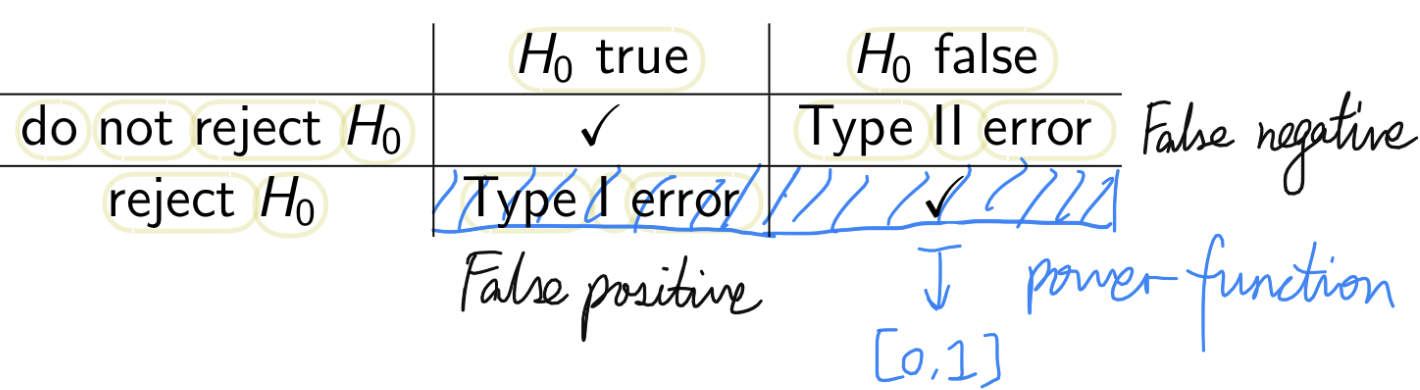
\includegraphics[scale=0.22]{./images/error_types.jpeg}
    \centering
    \caption{Type I and Type II errors}\label{error_types}
\end{figure}

\newtheorem{one-sided test eg}[theorem]{Example}
\begin{one-sided test eg}
    $X\sim\text{N}(\theta,1),\theta\in\mathbb{R}$ unknown. We test
    \[
        H_0:\theta\le 0\quad\text{against}\quad
        H_1:\theta>0.
    \]
    Thus $\Theta=\mathbb{R}$, $\Theta_0=(-\infty,0]$,
    $\Theta_1=(0,\infty)$. Suppose we use the critical (rejection) region
    \[
        R=[c,\infty).
    \]
    We choose a critical value $c$ s.t. the test is of level $\alpha$. For
    $\theta\le 0$:
    \[
        P_\theta(\text{reject }H_0)=P_\theta(X\ge c)
        =P_\theta(\underbrace{X-\theta}_{\sim\text{N}(0,1)}>c-\theta)
        =1-\Phi(c-\theta)\le 1-\Phi(c).
    \]
    Thus we choose $c$ s.t. $\Phi(c)=1-\alpha$, then
    $\forall\,\theta\in\Theta_0, P_\theta(\text{reject }H_0)\le\alpha$.
\end{one-sided test eg}

\section{Testing for a Population Mean}

Suppose $X_1,X_2,\ldots,X_n$ are i.i.d. N($\mu,\sigma^{2}$).
We wish to test if $\mu=\mu_0$ for some specific value
$\mu_0$, so we can state our null and alternative hypothesis as
\[
    H_0:\mu=\mu_0\quad\text{v.s.}\quad H_1:\mu\neq\mu_0
\]

\subsection{Normal Distribution with Known Variance}

Say $\sigma^2$ is known and $\mu$ is unknown.
We can set up a test statistic
\[
    Z=\frac{\overline{X}-\mu_0}{\frac{\sigma}{\sqrt{n}}}\sim\Phi.
\]
Thus the rejection region $R$ can be defined as
\[
    R = \left(-\infty,-z_{1-\frac{\alpha}{2}}\right)\cup
    \left(z_{1-\frac{\alpha}{2}},\infty\right)
    = \left\{z\big|\,|z|>z_{1-\frac{\alpha}{2}}\right\}
\]
s.t. $P(Z\in R|H_0)=\alpha$.
As such, we reject $H_0$ at the $\alpha$ significance level $\iff$ our observed
test statistic satisfies
\[
    z=\frac{\overline{x}-\mu_0}{\frac{\sigma}{\sqrt{n}}}\in R
    \quad\text{or}\quad
    p\text{-value}=2\left(1-\Phi(|z|)\right)\le\alpha.
\]

\subsection{Normal Distribution with Unknown Variance}

Say $\sigma^{2}$ is unknown and $\mu$ is unknown.
We can set up a test statistic
\[
    T=\frac{\overline{X}-\mu_0}{\frac{s_{n-1}}{\sqrt{n}}}\sim t_{n-1}.
\]
The rejection region $R$ thus changes to
\[
    R=\left\{t\big|\,|t|>t_{n-1,1-\frac{\alpha}{2}}\right\}
\]
s.t. $P(T\in R|H_0)=\alpha$.
As such, we reject $H_0$ at the $\alpha$ significance level $\iff$ our observed
test statistic satisfies
\[
    t=\frac{\overline{x}-\mu_0}{\frac{s_{n-1}}{\sqrt{n}}}\in R
    \quad\text{or}\quad
    p\text{-value}=2\left(1-t_{n-1, 1-\frac{\alpha}{2}}\right)\le\alpha.
\]

\section{Testing for Differences in Population Means}

Suppose that
\begin{itemize}
    \item $\mathbf{X}=(X_1,\ldots,X_{n_1})$ are i.i.d. N($\mu_X,\sigma_X^2$) with
        $\mu_X$ unknown;
    \item $\mathbf{Y}=(Y_1,\ldots,Y_{n_1})$ are i.i.d. N($\mu_Y,\sigma_Y^2$) with
        $\mu_Y$ unknown;
    \item the two samples $\mathbf{X}$ and $\mathbf{Y}$ are independent,
\end{itemize} 
and we want to test
\[
    H_0:\mu_X=\mu_Y\quad\text{v.s.}\quad
    H_1:\mu_X\neq\mu_Y.
\]

\subsection{Normal Distribution with Known Variances}

If $\sigma$ is known, we have
\[
    \overline{X}\sim\text{N}\left(\mu_X,\frac{\sigma_X^2}{n_1}\right),\quad
    \overline{Y}\sim\text{N}\left(\mu_Y,\frac{\sigma_Y^2}{n_1}\right)\quad
    \Longrightarrow\quad
    \overline{X}-\overline{Y}\sim\text{N}\left(\mu_X-\mu_Y,
    \frac{\sigma_X^2}{n_1}+\frac{\sigma_Y^2}{n_2}\right),
\]
thereby setting up test statistic
\[
    Z=\frac{(\overline{X}-\overline{Y})-(\mu_X-\mu_Y)}
    {\sqrt{\frac{\sigma_X^2}{n_1}+\frac{\sigma_Y^2}{n_2}}}
    =\frac{(\overline{X}-\overline{Y})}
    {\sqrt{\frac{\sigma_X^2}{n_1}+\frac{\sigma_Y^2}{n_2}}}
    \sim\Phi,
\]
following up with the investigation of rejection of null hypothesis.

\subsection{Normal Distribution with Unknown Variances}

If $\sigma$ is unknown, we have
\[
    T=\frac{(\overline{X}-\overline{Y})-(\mu_X-\mu_Y)}
    {S_{n_1+n_2-2}\sqrt{\frac{1}{n_1}+\frac{1}{n_2}}}
    =\frac{(\overline{X}-\overline{Y})}
    {S_{n_1+n_2-2}\sqrt{\frac{1}{n_1}+\frac{1}{n_2}}}
    \sim t_{n_1+n_2-2},
\]
following up with the investigation of rejection of null hypothesis.

\section{Goodness of Fit}

\subsection{Chi-square Test}

\newmdtheoremenv[style=defEnv]{chi-square statistic}[theorem]{Definition}
\begin{chi-square statistic}
    To test for \textbf{\emph{goodness of fit}}, i.e.\ compare the
    \emph{observed frequency} $\mathbf{O}=(O_1,\ldots,O_k)$ with the
    \emph{expected frequency} $\mathbb{E}=(E_1,\ldots,E_k)$, 
    we set up $H_0:\theta=\theta_0$ v.s. $H_1:\theta\neq\theta_0$ for the value
    of the unknown parameter, and use the \textbf{\emph{chi-square statistic}}
    \[
        \chi^2=\sum_{i=1}^{k} \frac{{(O_i-E_i)}^{2}}{E_i}. \quad(\ge 0)
    \]
    If $H_0$ were true, thenthe statistic $\chi^2$ would approximately follow a
    \textbf{\emph{chi-square distribution}} with $\nu=k-m-1$ degrees of freedom.
\end{chi-square statistic}
\paragraph{Comments}
\begin{itemize}
    \item $k$ is the number of values (categories) the simple random variable
        $X$ can take.
    \item $m$ is the number of parameters we needed to estimate from the data
        (dim($\theta$)) in order to calculate the $p_j$'s.
        \begin{itemize}
            \item E.g. given a sample without specifying the model, the degree
                of freedom $\nu=k-0-1=k-1$; if say the sample is fitted with a
                Poisson distribution with rate parameter $\lambda$, then
                $\nu=k-1-1=k-2$.
        \end{itemize} 
    \item For the approximation to be valid, we should have $\forall j,E_j\ge 5$.
        This may require some merging of categories.
    \item Larger $\chi^2$ corresponds to larger deviations from the null
        hypothesis model; if $\chi^2=0$, observed counts exactly match those
        expected under $H_0$.
    \item Since $\chi^2\ge 0$, we always perform a one-sided goodness of fit
        test using the $\chi^2$ statistic, looking at the upper tail of the
        distribution, leading to the rejection region $R$ at $\alpha$ level being
        \[
            R=\left\{x^{2}|x^{2}>\chi^2_{k-m-1,1-\alpha}\right\}.
        \]
\end{itemize} 

\subsection{Independence using Chi-square Statistic}

Assume two discrete random variables $X$ and $Y$ that can each take finite
values which are jointly distributed with unknown probability mass function
$p_{XY}$. To determine if $X$ and $Y$ are independent, we can do the following:

\bigskip
Let the ranges of $X$ and $Y$ be $\left\{x_1,\ldots,x_k\right\}$ and
$\left\{y_1,\ldots,y_l\right\}$ respectively.
Then we can form the following $k\times l$ \textbf{\emph{contingency table}}:
\begin{table}[h]
    \centering
    \caption{contingency table example}
    \label{contingency_table}
    \begin{tabular}{l|cccc|c}
        & $y_1$ & $y_2$ & \ldots & $y_l$ & \\
        \hline
        $x_1$ & $n_{11}$ & $n_{12}$ &   & $n_{1l}$ & $n_{1\bullet}$ \\
        $x_2$ & $n_{21}$ & $n_{22}$ &   & $n_{2l}$ & $n_{2\bullet}$ \\
        \vdots & & & & & \\
        $x_k$ & $n_{k1}$ & $n_{k 2}$ &   & $n_{kl}$ & $n_{k\bullet}$ \\
        \hline
              & $n_{\bullet 1}$ & $n_{\bullet 2}$ & \ldots & $n_{\bullet l}$ & $n$
    \end{tabular} 
\end{table} 

where $n_{ij}$ represents the number of times we observe the pair $(x_i,y_i)$,
$n_{i\bullet}$ represents the frequencies of $x_i$ in the sample, and similarly
for $n_{\bullet j}$. Under the null hypothesis,
\[
    H_0:\text{$X$ and $Y$ are independent},
\]
we can compute the expected values of entries of the contingency table by
\[
    \hat{n}_{ij}=\frac{n_{i\bullet}n_{\bullet j}}{n}
\]
since
\[
    \hat{p}_{i\bullet}=p_X(x_i)=\frac{n_{i\bullet}}{n},\quad
    \hat{p}_{\bullet j}=p_Y(y_j)=\frac{n_{\bullet j}}{n}\quad\Longrightarrow\quad
    \hat{p}_{ij}=\hat{p}_{i\bullet}\times \hat{p}_{\bullet j}
    =\frac{n_{i\bullet}n_{\bullet j}}{n^{2}}
\]
and multiply boths sides with $n$ to obtain the desired quantity $\hat{n}_{ij}$.
We can then set up the chi-square test statistic
\[
    x^2=\sum_{i,j}\frac{{(n_{ij}-\hat{n}_{ij})}^{2}}{\hat{n}_{ij}}
\]
with the degress of freedom $\nu=kl-(k-1)-(l-1)-1=(k-1)(l-1)$.
Hence the rejection region for a hypothesis test of independence in a $k\times
l$ contingency table at $\alpha$ level is given by
\[
    R=\left\{x^2|x^2>\chi^2_{(k-1)(l-1),1-\alpha}\right\}.
\]



\end{document}
